% Options for packages loaded elsewhere
\PassOptionsToPackage{unicode}{hyperref}
\PassOptionsToPackage{hyphens}{url}
%
\documentclass[
]{book}
\usepackage{amsmath,amssymb}
\usepackage{lmodern}
\usepackage{iftex}
\ifPDFTeX
  \usepackage[T1]{fontenc}
  \usepackage[utf8]{inputenc}
  \usepackage{textcomp} % provide euro and other symbols
\else % if luatex or xetex
  \usepackage{unicode-math}
  \defaultfontfeatures{Scale=MatchLowercase}
  \defaultfontfeatures[\rmfamily]{Ligatures=TeX,Scale=1}
\fi
% Use upquote if available, for straight quotes in verbatim environments
\IfFileExists{upquote.sty}{\usepackage{upquote}}{}
\IfFileExists{microtype.sty}{% use microtype if available
  \usepackage[]{microtype}
  \UseMicrotypeSet[protrusion]{basicmath} % disable protrusion for tt fonts
}{}
\makeatletter
\@ifundefined{KOMAClassName}{% if non-KOMA class
  \IfFileExists{parskip.sty}{%
    \usepackage{parskip}
  }{% else
    \setlength{\parindent}{0pt}
    \setlength{\parskip}{6pt plus 2pt minus 1pt}}
}{% if KOMA class
  \KOMAoptions{parskip=half}}
\makeatother
\usepackage{xcolor}
\usepackage{color}
\usepackage{fancyvrb}
\newcommand{\VerbBar}{|}
\newcommand{\VERB}{\Verb[commandchars=\\\{\}]}
\DefineVerbatimEnvironment{Highlighting}{Verbatim}{commandchars=\\\{\}}
% Add ',fontsize=\small' for more characters per line
\usepackage{framed}
\definecolor{shadecolor}{RGB}{248,248,248}
\newenvironment{Shaded}{\begin{snugshade}}{\end{snugshade}}
\newcommand{\AlertTok}[1]{\textcolor[rgb]{0.94,0.16,0.16}{#1}}
\newcommand{\AnnotationTok}[1]{\textcolor[rgb]{0.56,0.35,0.01}{\textbf{\textit{#1}}}}
\newcommand{\AttributeTok}[1]{\textcolor[rgb]{0.77,0.63,0.00}{#1}}
\newcommand{\BaseNTok}[1]{\textcolor[rgb]{0.00,0.00,0.81}{#1}}
\newcommand{\BuiltInTok}[1]{#1}
\newcommand{\CharTok}[1]{\textcolor[rgb]{0.31,0.60,0.02}{#1}}
\newcommand{\CommentTok}[1]{\textcolor[rgb]{0.56,0.35,0.01}{\textit{#1}}}
\newcommand{\CommentVarTok}[1]{\textcolor[rgb]{0.56,0.35,0.01}{\textbf{\textit{#1}}}}
\newcommand{\ConstantTok}[1]{\textcolor[rgb]{0.00,0.00,0.00}{#1}}
\newcommand{\ControlFlowTok}[1]{\textcolor[rgb]{0.13,0.29,0.53}{\textbf{#1}}}
\newcommand{\DataTypeTok}[1]{\textcolor[rgb]{0.13,0.29,0.53}{#1}}
\newcommand{\DecValTok}[1]{\textcolor[rgb]{0.00,0.00,0.81}{#1}}
\newcommand{\DocumentationTok}[1]{\textcolor[rgb]{0.56,0.35,0.01}{\textbf{\textit{#1}}}}
\newcommand{\ErrorTok}[1]{\textcolor[rgb]{0.64,0.00,0.00}{\textbf{#1}}}
\newcommand{\ExtensionTok}[1]{#1}
\newcommand{\FloatTok}[1]{\textcolor[rgb]{0.00,0.00,0.81}{#1}}
\newcommand{\FunctionTok}[1]{\textcolor[rgb]{0.00,0.00,0.00}{#1}}
\newcommand{\ImportTok}[1]{#1}
\newcommand{\InformationTok}[1]{\textcolor[rgb]{0.56,0.35,0.01}{\textbf{\textit{#1}}}}
\newcommand{\KeywordTok}[1]{\textcolor[rgb]{0.13,0.29,0.53}{\textbf{#1}}}
\newcommand{\NormalTok}[1]{#1}
\newcommand{\OperatorTok}[1]{\textcolor[rgb]{0.81,0.36,0.00}{\textbf{#1}}}
\newcommand{\OtherTok}[1]{\textcolor[rgb]{0.56,0.35,0.01}{#1}}
\newcommand{\PreprocessorTok}[1]{\textcolor[rgb]{0.56,0.35,0.01}{\textit{#1}}}
\newcommand{\RegionMarkerTok}[1]{#1}
\newcommand{\SpecialCharTok}[1]{\textcolor[rgb]{0.00,0.00,0.00}{#1}}
\newcommand{\SpecialStringTok}[1]{\textcolor[rgb]{0.31,0.60,0.02}{#1}}
\newcommand{\StringTok}[1]{\textcolor[rgb]{0.31,0.60,0.02}{#1}}
\newcommand{\VariableTok}[1]{\textcolor[rgb]{0.00,0.00,0.00}{#1}}
\newcommand{\VerbatimStringTok}[1]{\textcolor[rgb]{0.31,0.60,0.02}{#1}}
\newcommand{\WarningTok}[1]{\textcolor[rgb]{0.56,0.35,0.01}{\textbf{\textit{#1}}}}
\usepackage{longtable,booktabs,array}
\usepackage{calc} % for calculating minipage widths
% Correct order of tables after \paragraph or \subparagraph
\usepackage{etoolbox}
\makeatletter
\patchcmd\longtable{\par}{\if@noskipsec\mbox{}\fi\par}{}{}
\makeatother
% Allow footnotes in longtable head/foot
\IfFileExists{footnotehyper.sty}{\usepackage{footnotehyper}}{\usepackage{footnote}}
\makesavenoteenv{longtable}
\usepackage{graphicx}
\makeatletter
\def\maxwidth{\ifdim\Gin@nat@width>\linewidth\linewidth\else\Gin@nat@width\fi}
\def\maxheight{\ifdim\Gin@nat@height>\textheight\textheight\else\Gin@nat@height\fi}
\makeatother
% Scale images if necessary, so that they will not overflow the page
% margins by default, and it is still possible to overwrite the defaults
% using explicit options in \includegraphics[width, height, ...]{}
\setkeys{Gin}{width=\maxwidth,height=\maxheight,keepaspectratio}
% Set default figure placement to htbp
\makeatletter
\def\fps@figure{htbp}
\makeatother
\setlength{\emergencystretch}{3em} % prevent overfull lines
\providecommand{\tightlist}{%
  \setlength{\itemsep}{0pt}\setlength{\parskip}{0pt}}
\setcounter{secnumdepth}{5}
\usepackage{booktabs}
\ifLuaTeX
  \usepackage{selnolig}  % disable illegal ligatures
\fi
\usepackage[]{natbib}
\bibliographystyle{plainnat}
\IfFileExists{bookmark.sty}{\usepackage{bookmark}}{\usepackage{hyperref}}
\IfFileExists{xurl.sty}{\usepackage{xurl}}{} % add URL line breaks if available
\urlstyle{same} % disable monospaced font for URLs
\hypersetup{
  pdftitle={An Introduction to R for Quantitative Methods},
  pdfauthor={Brian Habing, Haley Jeppson},
  hidelinks,
  pdfcreator={LaTeX via pandoc}}

\title{An Introduction to R for Quantitative Methods}
\author{Brian Habing, Haley Jeppson}
\date{2023-04-05}

\begin{document}
\maketitle

{
\setcounter{tocdepth}{1}
\tableofcontents
}
\hypertarget{preface}{%
\chapter*{PREFACE}\label{preface}}
\addcontentsline{toc}{chapter}{PREFACE}

This book provides an introduction to R programming and serves as a companion to the data visualization workshop at NCME. It pulls from many sources, including \href{https://people.stat.sc.edu/habing/RforQM/RforQM.htm}{An Introduction to R for Quantitative Methods}, \href{https://r4ds.had.co.nz/}{R for Data Science}, \href{https://rstats.wtf/}{What They Forgot to Teach You About R}, \href{https://socviz.co/}{Data Visualization: A Practical Introduction}, \href{https://www.tmwr.org/}{Tidy Modeling with R}, and \href{https://stat480-at-isu.github.io/schedule.html}{Applied Statistical Computing}.

\hypertarget{conventions}{%
\section*{\texorpdfstring{Conventions\footnote{This section is repurposed from \href{https://socviz.co/}{Data Visualization: A Practical Introduction}}}{Conventions}}\label{conventions}}
\addcontentsline{toc}{section}{Conventions}

In this book, we alternate between regular text (like this), samples of code that you can type and run yourself, and the output of that code. In the main text, references to objects or other things that exist in the R language or in your R project---like tables of data, variables, functions, and so on---will also appear in \texttt{a\ monospaced} or \texttt{"typewriter"\ typeface}. Code you can type directly into R at the console will be in gray boxes, and also monospaced. Like this:

\begin{verbatim}
my_numbers <- c(1, 1, 4, 1, 1, 4, 1)
\end{verbatim}

If you type that line of code into R's console it will create a thing called \texttt{my\_numbers}. Doing this doesn't produce any output, however. When we write code that also produces output at the console, we will first see the code (in a gray box) and then the output in a monospaced font against a gray background. Here we add two numbers and see the result:

\begin{Shaded}
\begin{Highlighting}[]
\DecValTok{4} \SpecialCharTok{+} \DecValTok{1}
\end{Highlighting}
\end{Shaded}

\begin{verbatim}
## [1] 5
\end{verbatim}

Two further notes about how to read this. First, by default in this book, anything that comes back to us at the console as the result of typing a command will be shown prefaced by two hash characters (\texttt{\#\#}) at the beginning of each line of output. This is to help distinguish it from commands we type into the console. You will not see the hash characters at the console when you use R.

Second, both in the book \emph{and} at the console, if the output of what you did results in a series of elements (like numbers, or observations from a variable, and so on) you will often see output that includes some number in square brackets at the beginning of the line. It looks like this: \texttt{{[}1{]}}. This is not part of the output itself, but just a counter or index keeping track of how many items have been printed out so far. In the case of adding \texttt{4\ +\ 1} we got just one, or \texttt{{[}1{]}}, thing back---the number five. If there are more elements returned as the result of some instruction or command, the counter will keep track of that on each line. In this next bit of code we will tell R to show us the lower-case letters of the alphabet:

\begin{Shaded}
\begin{Highlighting}[]
\NormalTok{letters}
\end{Highlighting}
\end{Shaded}

\begin{verbatim}
##  [1] "a" "b" "c" "d" "e" "f" "g" "h" "i" "j" "k" "l" "m" "n" "o" "p" "q" "r" "s"
## [20] "t" "u" "v" "w" "x" "y" "z"
\end{verbatim}

You can see the counter incrementing on each line as it keeps count of how many letters have been printed.

\hypertarget{an-introduction}{%
\chapter{An Introduction}\label{an-introduction}}

\hypertarget{getting-started-in-r-with-rstudio}{%
\section*{Getting Started in R with RStudio}\label{getting-started-in-r-with-rstudio}}
\addcontentsline{toc}{section}{Getting Started in R with RStudio}

The book is designed for you to follow along in an active way, writing out the examples and experimenting with the code as you go. You will need to install some software first.

\hypertarget{r}{%
\subsection*{R}\label{r}}
\addcontentsline{toc}{subsection}{R}

R is based on the statistical programming language S and can be downloaded for free from \href{https://www.r-project.org/}{www.r-project.org}. Currently, to do so, choose: CRAN, then a mirror site in the US, then Download R for Windows, then base, then ``Download R 4.2.3 for Windows''. This page also has links to FAQs and other information about R.

R itself is a relatively small application with next to no user interface. Everything works through a command line, or console. At its most basic, you launch it from your Terminal application (on a Mac) or Command Prompt (on Windows) by typing \texttt{R}. Once launched, R awaits your instructions at a command line of its own, denoted by the right angle bracket symbol, \texttt{\textgreater{}}. When you type an instruction and hit return, R interprets it and sends any resulting output back to the console. But although a plain text file and a command line is the absolute minimum you need to work with R, it is a rather spartan arrangement. We can make life easier for ourselves by using RStudio.

\hypertarget{rstudio}{%
\subsection*{RStudio}\label{rstudio}}
\addcontentsline{toc}{subsection}{RStudio}

RStudio is an IDE (integrated development environment), and a convenient interface for R. Think of R as like a car's engine and RStudio as a car's dashboard. You can download and install Rstudio from the official \href{https://rstudio.com/products/rstudio/download/}{Rstudio website}. When launched, it starts up an instance of R's console inside of itself. It also conveniently pulls together various other elements to help you get your work done. These include the document where you are writing your code, the output it produces, and R's help system. RStudio also knows about RMarkdown, and understands a lot about the R language and the organization of your project.

Once you have both R and Rstudio installed, open Rstudio. You should now see four panels: (1) Source editor, (2) Console window,
(3) Environment pane, and
(4) Other tabs/panes.

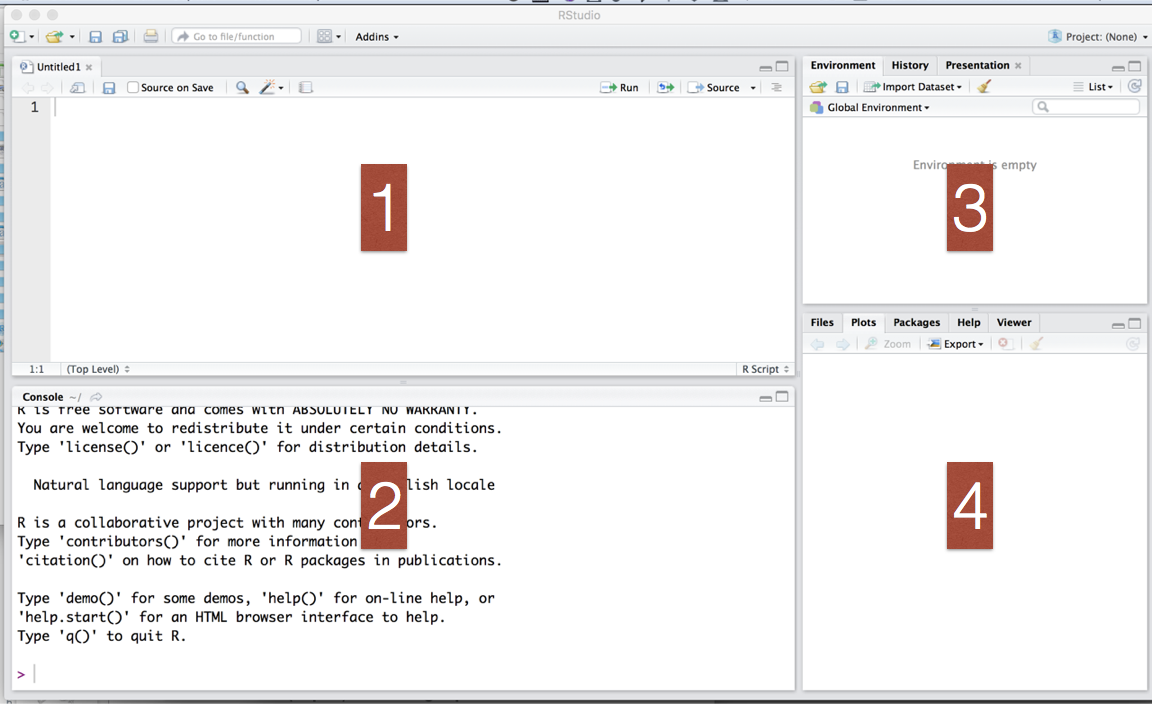
\includegraphics{img/rstudio-panes.png}

\hypertarget{executing-code-and-r-script-files}{%
\subsubsection*{Executing code and R script files}\label{executing-code-and-r-script-files}}
\addcontentsline{toc}{subsubsection}{Executing code and R script files}

You can start coding by typing commands in the \textbf{Console panel (2)}. This window is also where the output will appear. For example if you were to type 2+2 and hit return in that window it will return the answer 4.

When using the Console window in RStudio or R, the up and down-arrow on the key-board can be used to scroll through previously entered lines. \texttt{history()} will open a window of previously entered commands (which we'll see below after entering some). If the font in this R Console is too small, or if you dislike the color or font, you can change it by selecting ``Global Options'' under the ``Tools'' menu and clicking on the ``Appearance'' tab in the pop up window.

Because this Console window is used for so many things it often fills up quickly --- and so, if you are doing anything involving a large number of steps, it is often easiest to type them in a script first, which can be viewed in the \textbf{Source editor (1)}.

You can create a new script by clicking on the ``File'' menu and selecting ``New File'' then ``R Script''. A script is a collection of commands that you can save and run again later. To run a command, click in a given line or highlight the text and hit \texttt{Ctrl+Enter}, or click the ``Run'' button at the top of the script window. You can save your scripts for later use.

\hypertarget{packages}{%
\section{Packages}\label{packages}}

You'll also need to install some R packages. An R package is a collection of functions, data, and documentation that extends the capabilities of base R. Using packages is key to the successful use of R. For example, the \textbf{MASS} package contains all of the functions corresponding to the Springer text \emph{Modern Applied Statistics with S} by Venables and Ripley.

While some of these are automatically included with the basic installation of R, most are not and can installed with the \texttt{install.packages()} function.

\begin{Shaded}
\begin{Highlighting}[]
\FunctionTok{install.packages}\NormalTok{(}\StringTok{"package\_name"}\NormalTok{)}
\end{Highlighting}
\end{Shaded}

When you run the code to install a package on your own computer, R will download the packages from CRAN and install them on to your computer.

If you have problems installing, make sure that you are connected to the internet, and that \url{https://cloud.r-project.org/} isn't blocked by your firewall or proxy.

You will not be able to use the functions, objects, and help files in a package until you load it with \texttt{library()}.

\begin{Shaded}
\begin{Highlighting}[]
\FunctionTok{library}\NormalTok{(package\_name)}
\end{Highlighting}
\end{Shaded}

The command \texttt{library()} is used to activate a downloaded package and give access to all of its functions and must be done once per session.

\hypertarget{required-packages}{%
\subsection*{Required packages}\label{required-packages}}
\addcontentsline{toc}{subsection}{Required packages}

The remainder of this ebook (and the workshop) requires that you install the tidyverse library and several other add-on packages for R. These libraries provide useful functionality that we will take advantage of throughout the book. You can learn more about the tidyverse's family of packages at its website.

To install the necessary packages, type the following line of code at R's command prompt, located in the console window, and hit return.

\begin{Shaded}
\begin{Highlighting}[]
\FunctionTok{install.packages}\NormalTok{(}\StringTok{"tidyverse"}\NormalTok{)}
\end{Highlighting}
\end{Shaded}

R should then download and install these packages for you. It may take a little while to download everything.

Once you have installed the tidyverse package, you can load it with the \texttt{library()} function:

\begin{Shaded}
\begin{Highlighting}[]
\FunctionTok{library}\NormalTok{(tidyverse)}
\end{Highlighting}
\end{Shaded}

\hypertarget{objects}{%
\section{Objects}\label{objects}}

At the heart of R are the various objects that you enter. An object could be data (in the form of a single value, a vector, a matrix, an array, a list, or a data frame) or a function that you created. Objects are created by assigning a value to the objects name using either \texttt{\textless{}-} or \texttt{=}. For example

\begin{Shaded}
\begin{Highlighting}[]
\NormalTok{x }\OtherTok{\textless{}{-}} \DecValTok{3}
\end{Highlighting}
\end{Shaded}

All R statements where you create objects, \textbf{assignment statements}, have the same form:

\begin{Shaded}
\begin{Highlighting}[]
\NormalTok{object\_name }\OtherTok{\textless{}{-}}\NormalTok{ value}
\end{Highlighting}
\end{Shaded}

When reading that code say ``object name gets value'' in your head.

You will make lots of assignments, and \texttt{\textless{}-} is a pain to type. You can save time with \textbf{RStudio's keyboard shortcut: Alt + -} (the minus sign). Notice that RStudio automatically surrounds \texttt{\textless{}-} with spaces, which is a good code formatting practice. Code is miserable to read on a good day, so giveyoureyesabreak and use spaces.

If you run \texttt{x\ \textless{}-\ 3} in your local console (at the \texttt{\textgreater{}} prompt), R will only give you another prompt. This is because you merely assigned the value; you didn't ask R to do anything with it. Typing

\begin{Shaded}
\begin{Highlighting}[]
\NormalTok{x}
\end{Highlighting}
\end{Shaded}

\begin{verbatim}
## [1] 3
\end{verbatim}

will now return the number 3, the value of \texttt{x}. R is case sensitive, so entering \texttt{X\ \textless{}-\ 5} will create a separate object:

\begin{Shaded}
\begin{Highlighting}[]
\NormalTok{X }\OtherTok{\textless{}{-}} \DecValTok{5}
\NormalTok{X}
\end{Highlighting}
\end{Shaded}

\begin{verbatim}
## [1] 5
\end{verbatim}

If you reassign an object, say \texttt{X\ \textless{}-\ 7}, the original value is over-written:

\begin{Shaded}
\begin{Highlighting}[]
\NormalTok{X }\OtherTok{\textless{}{-}} \DecValTok{7}
\NormalTok{X}
\end{Highlighting}
\end{Shaded}

\begin{verbatim}
## [1] 7
\end{verbatim}

If you attempt to use the name of a built in function or constant (such as \texttt{c()}, \texttt{t()}, \texttt{t.test()}, or \texttt{pi()}) for one of your variable names, you will likely find that future work you are trying to do gives unexpected results. Notice in the name of \texttt{t.test()} that periods are allowed in names of objects. Other symbols (except numbers and letters) are not allowed.

\hypertarget{your-workspace}{%
\subsection*{Your workspace}\label{your-workspace}}
\addcontentsline{toc}{subsection}{Your workspace}

Note that the up-arrow and \texttt{history()} will now show us the commands we entered previously. This set of all of your created objects (your Workspace) is not saved by default when you exit R, and this is probably a good thing! Attachment to your workspace indicates that you have a \textbf{non-reproducible} workflow. Everything that really matters should be achieved through code that you save in your script, and so any individual R process and the associated workspace is disposable.

\begin{figure}
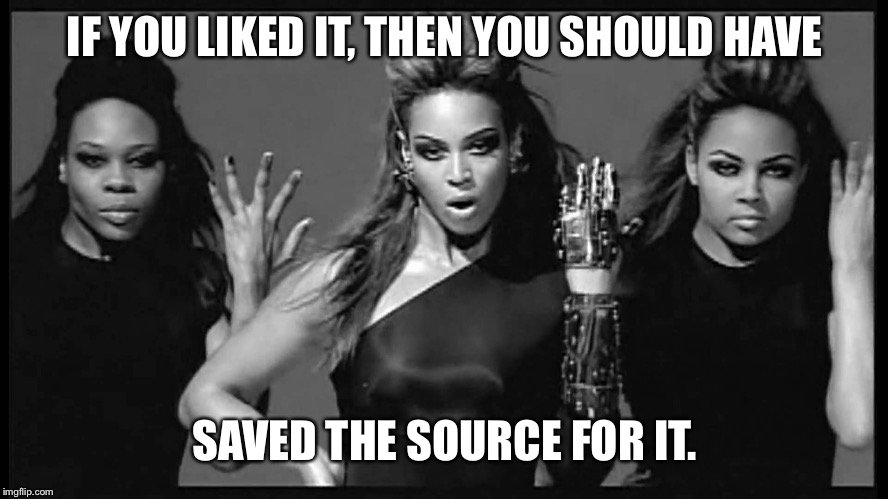
\includegraphics[width=12.33in]{img/if-you-liked-it-you-should-have-saved-the-source-for-it} \caption{ Image via Jenny Bryan's 'What They Forgot to Teach You About R'}\label{fig:unnamed-chunk-13}
\end{figure}

\hypertarget{data-types-in-r}{%
\subsection*{Data types in R}\label{data-types-in-r}}
\addcontentsline{toc}{subsection}{Data types in R}

R has a veriety of data types:

\begin{itemize}
\tightlist
\item
  \textbf{logical}: boolean values

  \begin{itemize}
  \tightlist
  \item
    ex. \texttt{TRUE} and \texttt{FALSE}
  \end{itemize}
\item
  \textbf{double}: floating point numerical values (default numerical type)

  \begin{itemize}
  \tightlist
  \item
    ex. \texttt{1.335} and \texttt{7}
  \end{itemize}
\item
  \textbf{integer}: integer numerical values (indicated with an L)

  \begin{itemize}
  \tightlist
  \item
    ex. \texttt{7L} and \texttt{1:3}
  \end{itemize}
\item
  \textbf{character}: character string

  \begin{itemize}
  \tightlist
  \item
    ex. \texttt{"hello"}\\
  \end{itemize}
\item
  \textbf{lists}: 1d objects that can contain any combination of R objects
\item
  \& more, but we won't be focusing on those yet
\end{itemize}

\hypertarget{arithmetic-and-parentheses}{%
\section{Arithmetic and Parentheses}\label{arithmetic-and-parentheses}}

Using R can be a lot like using a calculator. All of the basic arithmetic operations work in R:

\begin{Shaded}
\begin{Highlighting}[]
\NormalTok{X }\SpecialCharTok{{-}}\NormalTok{ x}
\end{Highlighting}
\end{Shaded}

\begin{verbatim}
## [1] 4
\end{verbatim}

\begin{Shaded}
\begin{Highlighting}[]
\DecValTok{7} \SpecialCharTok{{-}} \DecValTok{3}
\end{Highlighting}
\end{Shaded}

\begin{verbatim}
## [1] 4
\end{verbatim}

will both return the value 4, one by performing the arithmetic on the objects, and the other on the numbers. The other basic mathematical operators are:

\begin{itemize}
\tightlist
\item
  \texttt{+} addition
\item
  \texttt{-} subtraction
\item
  \texttt{*} multiplication
\item
  \texttt{/} division
\item
  \texttt{\^{}} exponentiation
\item
  \texttt{\%*\%} matrix multiplication
\end{itemize}

R will often try to do the ``common-sense'' thing when using arithmetic arguments. For example, if \texttt{Y} is a vector or matrix of values, then \texttt{Y\ +\ 4} will add \texttt{4} to each of the values in \texttt{Y}. (So the vector \texttt{3,\ 2,\ 5} would become \texttt{7,\ 6,\ 9}).

Parentheses work as usual in mathematical statements, but they do not imply multiplication.

\begin{Shaded}
\begin{Highlighting}[]
\FunctionTok{X}\NormalTok{(x}\SpecialCharTok{+}\DecValTok{5}\NormalTok{)}
\end{Highlighting}
\end{Shaded}

\begin{verbatim}
## Error in X(x + 5): could not find function "X"
\end{verbatim}

\begin{Shaded}
\begin{Highlighting}[]
\NormalTok{X}\SpecialCharTok{*}\NormalTok{(x}\SpecialCharTok{+}\DecValTok{5}\NormalTok{)}
\end{Highlighting}
\end{Shaded}

\begin{verbatim}
## [1] 56
\end{verbatim}

Notice that the former returns an error about looking for a function called \texttt{X}, while the latter does the arithmetic to return the value \texttt{40}.

The other use of parentheses in R are to indicate that you attempting to run a function, and, if the function has any options it will contain those. The command:

\begin{Shaded}
\begin{Highlighting}[]
\FunctionTok{rnorm}\NormalTok{(}\DecValTok{10}\NormalTok{)}
\end{Highlighting}
\end{Shaded}

\begin{verbatim}
##  [1] -0.83135745 -0.05771584  0.11992515  1.24019126  0.52583818  0.07892901
##  [7] -0.80854623 -1.40785156  0.27611173 -0.74571948
\end{verbatim}

runs the function \texttt{rnorm()} with the argument \texttt{10}. In this case it is generating a random sample of 10 values from a normal distribution.

\hypertarget{help}{%
\section{Help!}\label{help}}

To see this, we could run the help function on that command.

\begin{Shaded}
\begin{Highlighting}[]
\FunctionTok{help}\NormalTok{(rnorm)}
\end{Highlighting}
\end{Shaded}

A shortcut, \texttt{?rnorm}, would also work.

Every help file in R begins with a brief description of the function (or group of functions) in question, followed by all of the possible options (a.k.a. arguments) that you can provide. In this case the value \texttt{n} (the number of observations) is required. Notice that all of the other options are shown as being = some value -- this indicates the defaults those values take if you do not enter them. The sample we generated above thus has mean 0 and standard deviation 1.

Below the list of arguments are a brief summary of what the function does (called the \emph{Details}), a list of the \emph{Value} (or values) returned by running the function, the \emph{Source} of the algorithm, and general \emph{References} on the topic. \emph{See Also} is often the most useful part of the help for a function as it provides a list of related functions. Finally, there are some \emph{Examples} that you can cut and paste in to observe the function in action.

\hypertarget{functions}{%
\section{Functions}\label{functions}}

Functions are (most often) verbs, followed by what they will be applied to in parentheses:

\begin{Shaded}
\begin{Highlighting}[]
\FunctionTok{do\_this}\NormalTok{(to\_this)}
\FunctionTok{do\_that}\NormalTok{(to\_this, to\_that, with\_those)}
\end{Highlighting}
\end{Shaded}

It is always safest to enter the values of functions using the names of the arguments:

\begin{Shaded}
\begin{Highlighting}[]
\FunctionTok{rnorm}\NormalTok{(}\DecValTok{10}\NormalTok{, }\AttributeTok{sd =} \DecValTok{4}\NormalTok{)}
\end{Highlighting}
\end{Shaded}

\begin{verbatim}
##  [1]  4.5325259  3.3713886  0.5258709 -1.6386282 -2.9573859  5.5740353
##  [7]  4.0356427 -0.4743240  0.6558546  4.0589740
\end{verbatim}

rather than trusting that the argument you want happens to be first in the list:

\begin{Shaded}
\begin{Highlighting}[]
\FunctionTok{rnorm}\NormalTok{(}\DecValTok{10}\NormalTok{, }\DecValTok{4}\NormalTok{)}
\end{Highlighting}
\end{Shaded}

\begin{verbatim}
##  [1] 4.110017 2.665559 3.515594 3.806785 4.286762 5.155799 4.107901 4.934832
##  [9] 3.335690 4.671638
\end{verbatim}

Notice the former puts 4 in for the standard deviation, while the latter is putting it in for the second overall argument, the mean (as seen in the help file).

Note that these values we generated have not been saved as an object, and exist solely on the screen. To save the values we could have assigned the output of our function to an object.

\begin{Shaded}
\begin{Highlighting}[]
\NormalTok{normal.sample }\OtherTok{\textless{}{-}} \FunctionTok{rnorm}\NormalTok{(}\DecValTok{50}\NormalTok{)}
\NormalTok{normal.sample}
\end{Highlighting}
\end{Shaded}

\begin{verbatim}
##  [1] -1.174014066 -0.429539926  0.745276755  0.309033224 -0.634503827
##  [6] -0.598959370 -0.251471782 -0.632227528 -0.187702052  0.343233784
## [11] -1.366639789 -2.211957746 -1.267110111  0.586223011 -1.663638587
## [16] -0.383819100  0.369547870  0.558477157 -0.283246447  0.021109599
## [21]  0.277279915 -0.473821362  0.104009665 -1.579748150 -0.436807159
## [26] -0.061014523 -0.313337810 -0.087675795 -0.144332371  0.547900841
## [31] -1.303449192  1.525693289 -1.154091998 -1.510236247 -0.439333099
## [36] -0.031247707  0.003400634 -1.117729954  0.369133408 -1.272193212
## [41]  0.002192800 -0.595842547  2.007211234 -0.232934031  0.054203535
## [46] -0.899125812  1.554486024 -0.605380227  0.154376702 -1.132004017
\end{verbatim}

\hypertarget{common-statistical-functions}{%
\subsection*{Common statistical functions}\label{common-statistical-functions}}
\addcontentsline{toc}{subsection}{Common statistical functions}

A few common statistical functions include:

\begin{itemize}
\tightlist
\item
  \texttt{mean()} find the mean
\item
  \texttt{median()} find the median
\item
  \texttt{sd()} find the standard deviation
\item
  \texttt{var()} find the variance
\item
  \texttt{quantile()} find the quantiles (percentiles);

  \begin{itemize}
  \tightlist
  \item
    requires the data and the percentile you want
  \item
    e.g.~\texttt{quantile(normal.sample,\ .5)} is the median
  \end{itemize}
\item
  \texttt{max()} find the maximum
\item
  \texttt{min()} find the minimum
\item
  \texttt{summary()} find the 5-number summary
\item
  \texttt{hist()} construct a histogram
\item
  \texttt{boxplot()} construct a boxplot
\item
  \texttt{qqnorm()} construct a normal quantile-quantile plot
\item
  \texttt{qqline()} add the line to a normal quantile-quantile plot
\end{itemize}

Trying a few of these out (like \texttt{mean(normal.sample)}) will show us the descriptive statistics and basic graphs for a sample of size 50 from a normal population with mean 0 and standard deviation 1. (Using up arrow can make it quicker to try several in a row.)

As we will see in more detail later, it is possible to create your own functions by using the function function. This one creates a simple measure of skewness.

\begin{Shaded}
\begin{Highlighting}[]
\NormalTok{Skew }\OtherTok{\textless{}{-}} \ControlFlowTok{function}\NormalTok{(x)\{}
\NormalTok{    (}\FunctionTok{mean}\NormalTok{(x) }\SpecialCharTok{{-}} \FunctionTok{median}\NormalTok{(x))}\SpecialCharTok{/}\FunctionTok{sd}\NormalTok{(x)\}}
\end{Highlighting}
\end{Shaded}

Note that braces \texttt{\{\ \}} in R are used to group several separate commands together, and also occur when using programming commands like loops or if-then statements. They work the same as parentheses in arithmetic expressions.

After entering or new function, it works like any built in function, except that it appears in our objects list.

\begin{Shaded}
\begin{Highlighting}[]
\NormalTok{Skew}
\end{Highlighting}
\end{Shaded}

\begin{verbatim}
## function(x){
##     (mean(x) - median(x))/sd(x)}
\end{verbatim}

\begin{Shaded}
\begin{Highlighting}[]
\FunctionTok{Skew}\NormalTok{()}
\end{Highlighting}
\end{Shaded}

\begin{verbatim}
## Error in mean(x): argument "x" is missing, with no default
\end{verbatim}

\begin{Shaded}
\begin{Highlighting}[]
\FunctionTok{Skew}\NormalTok{(normal.sample)}
\end{Highlighting}
\end{Shaded}

\begin{verbatim}
## [1] -0.03731881
\end{verbatim}

\hypertarget{common-mathematical-functions}{%
\subsection*{Common mathematical functions}\label{common-mathematical-functions}}
\addcontentsline{toc}{subsection}{Common mathematical functions}

There are also a number of mathematical functions as well. Ones common in statistical applications include:

\begin{itemize}
\tightlist
\item
  \texttt{sqrt()} square root
\item
  \texttt{exp()} exponent (e to the power)
\item
  \texttt{log()} the natural logarithm by default
\item
  \texttt{abs()} absolute values
\item
  \texttt{floor()} round down
\item
  \texttt{ceiling()} round up
\item
  \texttt{round()} round to the nearest (even if .5)
\end{itemize}

\hypertarget{vectors-matrices-and-arrays}{%
\section{Vectors, Matrices, and Arrays}\label{vectors-matrices-and-arrays}}

\hypertarget{vectors}{%
\subsection*{Vectors}\label{vectors}}
\addcontentsline{toc}{subsection}{Vectors}

The output from \texttt{rnorm()} is different from the \texttt{X} and \texttt{x} we created as it contains more than just a single value - they are vectors. While we can think of them as vectors in the mathematical sense, we can also think of a vector as simply listing the values of a variable.

Vectors in R are created using the \texttt{c()} function (as in concatonate). Thus,

\begin{Shaded}
\begin{Highlighting}[]
\NormalTok{Y }\OtherTok{\textless{}{-}} \FunctionTok{c}\NormalTok{(}\DecValTok{3}\NormalTok{, }\DecValTok{2}\NormalTok{, }\DecValTok{5}\NormalTok{)}
\NormalTok{Y}
\end{Highlighting}
\end{Shaded}

\begin{verbatim}
## [1] 3 2 5
\end{verbatim}

\begin{Shaded}
\begin{Highlighting}[]
\NormalTok{Y }\SpecialCharTok{+} \DecValTok{4}
\end{Highlighting}
\end{Shaded}

\begin{verbatim}
## [1] 7 6 9
\end{verbatim}

\begin{Shaded}
\begin{Highlighting}[]
\NormalTok{Y }\SpecialCharTok{*} \DecValTok{2}
\end{Highlighting}
\end{Shaded}

\begin{verbatim}
## [1]  6  4 10
\end{verbatim}

creates a vector of length three (and we can verify that arithmetic works on it componentwise). Given two vectors arithmetic is also done componentwise:

\begin{Shaded}
\begin{Highlighting}[]
\NormalTok{Z }\OtherTok{\textless{}{-}} \FunctionTok{c}\NormalTok{(}\DecValTok{1}\NormalTok{, }\DecValTok{2}\NormalTok{, }\DecValTok{3}\NormalTok{)}
\NormalTok{Y }\SpecialCharTok{+}\NormalTok{ Z}
\end{Highlighting}
\end{Shaded}

\begin{verbatim}
## [1] 4 4 8
\end{verbatim}

\begin{Shaded}
\begin{Highlighting}[]
\NormalTok{Y }\SpecialCharTok{*}\NormalTok{ Z}
\end{Highlighting}
\end{Shaded}

\begin{verbatim}
## [1]  3  4 15
\end{verbatim}

Other functions are also evaluated component-wise (if possible):

\begin{Shaded}
\begin{Highlighting}[]
\FunctionTok{sqrt}\NormalTok{(Z)}
\end{Highlighting}
\end{Shaded}

\begin{verbatim}
## [1] 1.000000 1.414214 1.732051
\end{verbatim}

Multiple vectors can be combined together by using the \texttt{c()} function:

\begin{Shaded}
\begin{Highlighting}[]
\NormalTok{YandZ }\OtherTok{\textless{}{-}} \FunctionTok{c}\NormalTok{(Y, Z)}
\NormalTok{YandZ}
\end{Highlighting}
\end{Shaded}

\begin{verbatim}
## [1] 3 2 5 1 2 3
\end{verbatim}

However, when asked to combine vectors of two different types, R will try to force them to be of the same type:

\begin{Shaded}
\begin{Highlighting}[]
\NormalTok{nums }\OtherTok{\textless{}{-}} \FunctionTok{c}\NormalTok{(}\DecValTok{1}\NormalTok{, }\DecValTok{2}\NormalTok{, }\DecValTok{3}\NormalTok{)}
\NormalTok{nums}
\end{Highlighting}
\end{Shaded}

\begin{verbatim}
## [1] 1 2 3
\end{verbatim}

\begin{Shaded}
\begin{Highlighting}[]
\NormalTok{lttrs }\OtherTok{\textless{}{-}} \FunctionTok{c}\NormalTok{(}\StringTok{"a"}\NormalTok{, }\StringTok{"b"}\NormalTok{, }\StringTok{"c"}\NormalTok{)}
\NormalTok{lttrs}
\end{Highlighting}
\end{Shaded}

\begin{verbatim}
## [1] "a" "b" "c"
\end{verbatim}

\begin{Shaded}
\begin{Highlighting}[]
\FunctionTok{c}\NormalTok{(nums, lttrs)}
\end{Highlighting}
\end{Shaded}

\begin{verbatim}
## [1] "1" "2" "3" "a" "b" "c"
\end{verbatim}

\begin{Shaded}
\begin{Highlighting}[]
\FunctionTok{c}\NormalTok{(nums, lttrs) }\SpecialCharTok{+} \DecValTok{2}
\end{Highlighting}
\end{Shaded}

\begin{verbatim}
## Error in c(nums, lttrs) + 2: non-numeric argument to binary operator
\end{verbatim}

Once we have our desired vector, an element in the vector can be referred to by using square brackets:

\begin{Shaded}
\begin{Highlighting}[]
\NormalTok{YandZ[}\DecValTok{2}\NormalTok{]}
\end{Highlighting}
\end{Shaded}

\begin{verbatim}
## [1] 2
\end{verbatim}

\begin{Shaded}
\begin{Highlighting}[]
\NormalTok{YandZ[}\DecValTok{2}\SpecialCharTok{:}\DecValTok{4}\NormalTok{]}
\end{Highlighting}
\end{Shaded}

\begin{verbatim}
## [1] 2 5 1
\end{verbatim}

\begin{Shaded}
\begin{Highlighting}[]
\NormalTok{YandZ[}\FunctionTok{c}\NormalTok{(}\DecValTok{1}\NormalTok{, }\DecValTok{4}\SpecialCharTok{:}\DecValTok{6}\NormalTok{)]}
\end{Highlighting}
\end{Shaded}

\begin{verbatim}
## [1] 3 1 2 3
\end{verbatim}

By using the \texttt{c()} function, and the \texttt{:} to indicate a sequence of numbers, you can quickly refer to the particular portion of the data you are concerned with.

\hypertarget{matrices-and-arrays}{%
\subsection*{Matrices and arrays}\label{matrices-and-arrays}}
\addcontentsline{toc}{subsection}{Matrices and arrays}

Matrices (two-dimensional) and arrays (more than two dimensions) work similarly - they use brackets to find particular values, and all the values in an array or matrix must be of the same type (e.g.~numeric, character, or factor). In the case of matrices, the first values in the brackets indicates the desired rows, and the ones after the comma indicate the desired columns.

\begin{Shaded}
\begin{Highlighting}[]
\NormalTok{Xmat }\OtherTok{\textless{}{-}} \FunctionTok{matrix}\NormalTok{(}\FunctionTok{c}\NormalTok{(}\DecValTok{3}\NormalTok{, }\DecValTok{2}\NormalTok{, }\DecValTok{5}\NormalTok{, }\DecValTok{1}\NormalTok{, }\DecValTok{2}\NormalTok{, }\DecValTok{3}\NormalTok{), }
               \AttributeTok{ncol =} \DecValTok{3}\NormalTok{, }\AttributeTok{byrow =} \ConstantTok{TRUE}\NormalTok{)}
\NormalTok{Xmat}
\end{Highlighting}
\end{Shaded}

\begin{verbatim}
##      [,1] [,2] [,3]
## [1,]    3    2    5
## [2,]    1    2    3
\end{verbatim}

\begin{Shaded}
\begin{Highlighting}[]
\NormalTok{Ymat }\OtherTok{\textless{}{-}} \FunctionTok{rbind}\NormalTok{(Y, Z)}
\NormalTok{Ymat}
\end{Highlighting}
\end{Shaded}

\begin{verbatim}
##   [,1] [,2] [,3]
## Y    3    2    5
## Z    1    2    3
\end{verbatim}

\begin{Shaded}
\begin{Highlighting}[]
\NormalTok{Xmat[}\DecValTok{1}\NormalTok{, }\DecValTok{2}\SpecialCharTok{:}\DecValTok{3}\NormalTok{]}
\end{Highlighting}
\end{Shaded}

\begin{verbatim}
## [1] 2 5
\end{verbatim}

\begin{Shaded}
\begin{Highlighting}[]
\NormalTok{Zmat }\OtherTok{\textless{}{-}} \FunctionTok{cbind}\NormalTok{(nums, lttrs)}
\NormalTok{Zmat}
\end{Highlighting}
\end{Shaded}

\begin{verbatim}
##      nums lttrs
## [1,] "1"  "a"  
## [2,] "2"  "b"  
## [3,] "3"  "c"
\end{verbatim}

In the above code, \texttt{matrix()} is the function to form a vector into a matrix, \texttt{rbind()} places multiple vectors (or matrices) side-by-side as the rows of a new matrix (if the dimensions match), and \texttt{cbind()} does the same for columns.

\hypertarget{data-frames-lists-and-attributes}{%
\section{Data Frames, Lists, and Attributes}\label{data-frames-lists-and-attributes}}

\hypertarget{data-frames}{%
\subsection*{Data frames}\label{data-frames}}
\addcontentsline{toc}{subsection}{Data frames}

In many cases the data set we wish to analyze will not have all of the rows or columns in the same format. This type of data is stored in R as a \textbf{data frame}. A data frame is a rectangular collection of variables (in the columns) and observations (in the rows).

\texttt{scdata.txt} is one such data set, and it can be found in the course materials (its description is found in \texttt{scdata.pdf}). The data can be read in using code similar to the below (assuming a similar file structure).

\begin{Shaded}
\begin{Highlighting}[]
\NormalTok{url }\OtherTok{\textless{}{-}} \StringTok{"https://people.stat.sc.edu/habing/RforQM/scdata.txt"}
\NormalTok{sctable }\OtherTok{\textless{}{-}}\NormalTok{ readr}\SpecialCharTok{::}\FunctionTok{read\_table}\NormalTok{(url)}
\end{Highlighting}
\end{Shaded}

The function \texttt{read\_table()} reads in our file as a \textbf{tibble}, unlike \texttt{read.table()} which reads in the file as R's traditional \texttt{data.table}. Tibbles are data frames, but more opinionated, and they tweak some older behaviors to make working in the tidyverse a little easier.

There are a few good reasons to favor \textbf{\{readr\}} functions over the base equivalents:

\begin{itemize}
\item
  They are typically much faster than their base equivalents. Long running jobs have a progress bar, so you can see what's happening. If you're looking for raw speed, try \texttt{data.table::fread()}. It doesn't fit quite so well into the tidyverse, but it can be quite a bit faster.
\item
  They produce tibbles, they don't convert character vectors to factors, use row names, or munge the column names. These are common sources of frustration with the base R functions.
\item
  They are more reproducible. Base R functions inherit some behavior from your operating system and environment variables, so import code that works on your computer might not work on someone else's.
\item
  Tibbles are designed so that you don't accidentally overwhelm your console when you print large data frames.
\end{itemize}

Some older functions don't work with tibbles. If you encounter one of these functions, use \texttt{as.data.frame()} to turn a tibble back to a data.frame. The main reason that some older functions don't work with tibble is the \texttt{{[}} function. With base R data frames, \texttt{{[}} sometimes returns a data frame, and sometimes returns a vector. With tibbles, \texttt{{[}} always returns another tibble.

\hypertarget{inspecting-objects}{%
\subsection*{Inspecting objects}\label{inspecting-objects}}
\addcontentsline{toc}{subsection}{Inspecting objects}

To inspect the data without needing to print out the entire data set, we can try out the following commands:

\begin{itemize}
\tightlist
\item
  \texttt{head()}
\item
  \texttt{tail()}
\item
  \texttt{summary()}
\item
  \texttt{str()}
\item
  \texttt{dim()}
\end{itemize}

For example, use \texttt{head()} and \texttt{tail()} to see the first and last rows. This lets you check the variable names as well as the number of observations successfully read in.

\begin{Shaded}
\begin{Highlighting}[]
\FunctionTok{head}\NormalTok{(sctable)}
\end{Highlighting}
\end{Shaded}

\begin{verbatim}
## # A tibble: 6 x 27
##   County Region Births Death InfMort Minor~1 Over65 PopChng PopDens Urban Income
##   <chr>  <chr>   <dbl> <dbl>   <dbl>   <dbl>  <dbl>   <dbl>   <dbl> <dbl>  <dbl>
## 1 Abbev~ Upsta~   12.5  10.3    15.1    31.7   14.7     9.7    51.5  23.4  32635
## 2 Aiken  Midla~   12.1   9.8     9.6    28.6   12.8    17.8   133.   60.9  37889
## 3 Allen~ LowCo~   14.8  12.1    18.5    72.6   12.7    -4.4    27.5  59    20898
## 4 Ander~ Upsta~   13    10.7    10.3    18.4   13.7    14.2   231.   58.3  36807
## 5 Bambe~ Midla~   11.5   9.9    21.7    63.5   13.9    -1.4    42.4  45.7  24007
## 6 Barnw~ Midla~   14    10.9    21.4    44.8   12.6    15.7    42.8  14.9  28591
## # ... with 16 more variables: ConsInc <dbl>, FarmInc <dbl>, ManIncom <dbl>,
## #   RetInc <dbl>, FdStmps <dbl>, MoblHms <dbl>, NoCar <dbl>, PlumProb <dbl>,
## #   PoorChild <dbl>, Unemp <dbl>, Coll4 <dbl>, Crime <dbl>, HSGrad <dbl>,
## #   JuvDel <dbl>, MVDeath <dbl>, SchlSpnd <dbl>, and abbreviated variable name
## #   1: Minority
\end{verbatim}

\begin{Shaded}
\begin{Highlighting}[]
\FunctionTok{tail}\NormalTok{(sctable)}
\end{Highlighting}
\end{Shaded}

\begin{verbatim}
## # A tibble: 6 x 27
##   County Region Births Death InfMort Minor~1 Over65 PopChng PopDens Urban Income
##   <chr>  <chr>   <dbl> <dbl>   <dbl>   <dbl>  <dbl>   <dbl>   <dbl> <dbl>  <dbl>
## 1 Saluda Midla~   11.2  11.3     4.7    34.2   14.5    16.7    42.5  18.7  35774
## 2 Spart~ Upsta~   13.1   9.8     7.9    24.9   12.5    11.9   313.   64.8  37579
## 3 Sumter Midla~   15.6   8.9     8.5    50     11.2     3.3   157.   62.1  33278
## 4 Union  Upsta~   10.7  13.2    12.8    32.2   15.6    -1.5    58.1  35.7  31441
## 5 Willi~ Peedee   12.6  11.8     8.8    67.3   13       1.1    39.8  15.1  24214
## 6 York   Upsta~   13.4   7.7     7.6    22.7   10.4    25.2   241.   64.3  44539
## # ... with 16 more variables: ConsInc <dbl>, FarmInc <dbl>, ManIncom <dbl>,
## #   RetInc <dbl>, FdStmps <dbl>, MoblHms <dbl>, NoCar <dbl>, PlumProb <dbl>,
## #   PoorChild <dbl>, Unemp <dbl>, Coll4 <dbl>, Crime <dbl>, HSGrad <dbl>,
## #   JuvDel <dbl>, MVDeath <dbl>, SchlSpnd <dbl>, and abbreviated variable name
## #   1: Minority
\end{verbatim}

\hypertarget{extracting-parts-of-objects}{%
\subsection*{Extracting parts of objects}\label{extracting-parts-of-objects}}
\addcontentsline{toc}{subsection}{Extracting parts of objects}

For object \texttt{x}, we can extract parts in the following manner (\texttt{rows} and \texttt{columns} are vectors of indices):

\begin{Shaded}
\begin{Highlighting}[]
\NormalTok{x}\SpecialCharTok{$}\NormalTok{variable}
\NormalTok{x[, }\StringTok{"variable"}\NormalTok{]}
\NormalTok{x[rows, columns]}
\NormalTok{x[}\DecValTok{1}\SpecialCharTok{:}\DecValTok{5}\NormalTok{, }\DecValTok{2}\SpecialCharTok{:}\DecValTok{3}\NormalTok{]}
\NormalTok{x[}\FunctionTok{c}\NormalTok{(}\DecValTok{1}\NormalTok{,}\DecValTok{5}\NormalTok{,}\DecValTok{6}\NormalTok{), }\FunctionTok{c}\NormalTok{(}\StringTok{"County"}\NormalTok{, }\StringTok{"Region"}\NormalTok{)]}
\NormalTok{x}\SpecialCharTok{$}\NormalTok{variable[rows]}
\end{Highlighting}
\end{Shaded}

Many of these extraction methods access the rows and columns of a data frame by treating it similarly to a matrix:

\begin{Shaded}
\begin{Highlighting}[]
\NormalTok{County1 }\OtherTok{\textless{}{-}}\NormalTok{ sctable[}\DecValTok{1}\NormalTok{, ]}
\NormalTok{Birth.Death }\OtherTok{\textless{}{-}}\NormalTok{ sctable[ , }\DecValTok{3}\SpecialCharTok{:}\DecValTok{4}\NormalTok{]}
\end{Highlighting}
\end{Shaded}

This simplicity sometimes causes trouble though. While \texttt{Birth.Death} may look on the screen like it is a matrix, it is still a data frame and many functions which use matrix operations (like matrix multiplication) will give an error. The \texttt{attributes()} function will show us the true status of our object (it returns \texttt{NULL} for a numeric vector and the dimensions if a matrix):

\begin{Shaded}
\begin{Highlighting}[]
\NormalTok{Birth.Death}
\end{Highlighting}
\end{Shaded}

\begin{verbatim}
## # A tibble: 46 x 2
##    Births Death
##     <dbl> <dbl>
##  1   12.5  10.3
##  2   12.1   9.8
##  3   14.8  12.1
##  4   13    10.7
##  5   11.5   9.9
##  6   14    10.9
##  7   15.8   7.8
##  8   14.4   6.6
##  9   11.5  11.1
## 10   14.5   8.5
## # ... with 36 more rows
\end{verbatim}

\begin{Shaded}
\begin{Highlighting}[]
\FunctionTok{attributes}\NormalTok{(Birth.Death)}
\end{Highlighting}
\end{Shaded}

\begin{verbatim}
## $names
## [1] "Births" "Death" 
## 
## $row.names
##  [1]  1  2  3  4  5  6  7  8  9 10 11 12 13 14 15 16 17 18 19 20 21 22 23 24 25
## [26] 26 27 28 29 30 31 32 33 34 35 36 37 38 39 40 41 42 43 44 45 46
## 
## $class
## [1] "tbl_df"     "tbl"        "data.frame"
\end{verbatim}

\begin{Shaded}
\begin{Highlighting}[]
\NormalTok{BD.matrix }\OtherTok{\textless{}{-}} \FunctionTok{as.matrix}\NormalTok{(Birth.Death)}
\FunctionTok{attributes}\NormalTok{(BD.matrix)}
\end{Highlighting}
\end{Shaded}

\begin{verbatim}
## $dim
## [1] 46  2
## 
## $dimnames
## $dimnames[[1]]
## NULL
## 
## $dimnames[[2]]
## [1] "Births" "Death"
\end{verbatim}

The \texttt{\$} is used to access whatever corresponds to an entry in the names attribute:

\begin{Shaded}
\begin{Highlighting}[]
\NormalTok{Birth.Death}\SpecialCharTok{$}\NormalTok{Births}
\end{Highlighting}
\end{Shaded}

\begin{verbatim}
##  [1] 12.5 12.1 14.8 13.0 11.5 14.0 15.8 14.4 11.5 14.5 13.3 12.3 12.1 12.3 13.0
## [16] 12.4 15.6 12.9 10.3 12.8 15.3 12.7 14.0 12.6 13.9 12.7 14.3 12.8 12.2 11.6
## [31] 12.9 14.0  7.6 13.8 11.9 12.5 11.7 13.8 11.2 13.3 11.2 13.1 15.6 10.7 12.6
## [46] 13.4
\end{verbatim}

This is particularly useful when trying to access a portion of the output of a function for later use. For example, later we will see a method of doing statistical inference called the t-test. In R, this is performed by the function \texttt{t.test()} which can create a great deal of output on the screen.

\begin{Shaded}
\begin{Highlighting}[]
\FunctionTok{t.test}\NormalTok{(normal.sample)}
\end{Highlighting}
\end{Shaded}

\begin{verbatim}
## 
##  One Sample t-test
## 
## data:  normal.sample
## t = -2.5045, df = 49, p-value = 0.01564
## alternative hypothesis: true mean is not equal to 0
## 95 percent confidence interval:
##  -0.53863851 -0.05905534
## sample estimates:
##  mean of x 
## -0.2988469
\end{verbatim}

If you only want the part called the ``p-value'' for later use we can pull that out of the output.

\begin{Shaded}
\begin{Highlighting}[]
\NormalTok{t.out }\OtherTok{\textless{}{-}} \FunctionTok{t.test}\NormalTok{(normal.sample)}
\FunctionTok{attributes}\NormalTok{(t.out)}
\end{Highlighting}
\end{Shaded}

\begin{verbatim}
## $names
##  [1] "statistic"   "parameter"   "p.value"     "conf.int"    "estimate"   
##  [6] "null.value"  "stderr"      "alternative" "method"      "data.name"  
## 
## $class
## [1] "htest"
\end{verbatim}

\begin{Shaded}
\begin{Highlighting}[]
\NormalTok{t.out}\SpecialCharTok{$}\NormalTok{p.value}
\end{Highlighting}
\end{Shaded}

\begin{verbatim}
## [1] 0.01563949
\end{verbatim}

We could then save the resulting value as part of a vector or matrix of other p-values, for example.

The \texttt{\$} is also used to access named parts of lists, which we will see can be used to store a variety of kinds of information in a single object.

\hypertarget{rmarkdown}{%
\section{RMarkdown}\label{rmarkdown}}

Beyond data analysis, coding, and creating graphics, R and RStudio also allow for the creation of documents using Markdown. Markdown is a particular type of markup language. Markup languages are designed to produce documents from plain text. Some of you may be familiar with LaTeX, another (less human friendly) markup language for creating pdf documents. LaTeX gives you much greater control, but it is restricted to pdf and has a much greater learning curve.

Markdown is becoming a standard and many websites will generate HTML from Markdown (e.g.~GitHub, Stack Overflow, reddit, \ldots). It is also relatively easy:

\begin{verbatim}
*italic*
**bold**
# Header 1
## Header 2
### Header 3
- List item 1
- List item 2
    - item 2a
    - item 2b
1. Numbered list item 1
1. Numbered list item 2
    - item 2a
    - item 2b
\end{verbatim}

Have a look at RStudio's \href{https://www.rstudio.com/resources/cheatsheets/}{RMarkdown cheat sheet}.

\begin{figure}
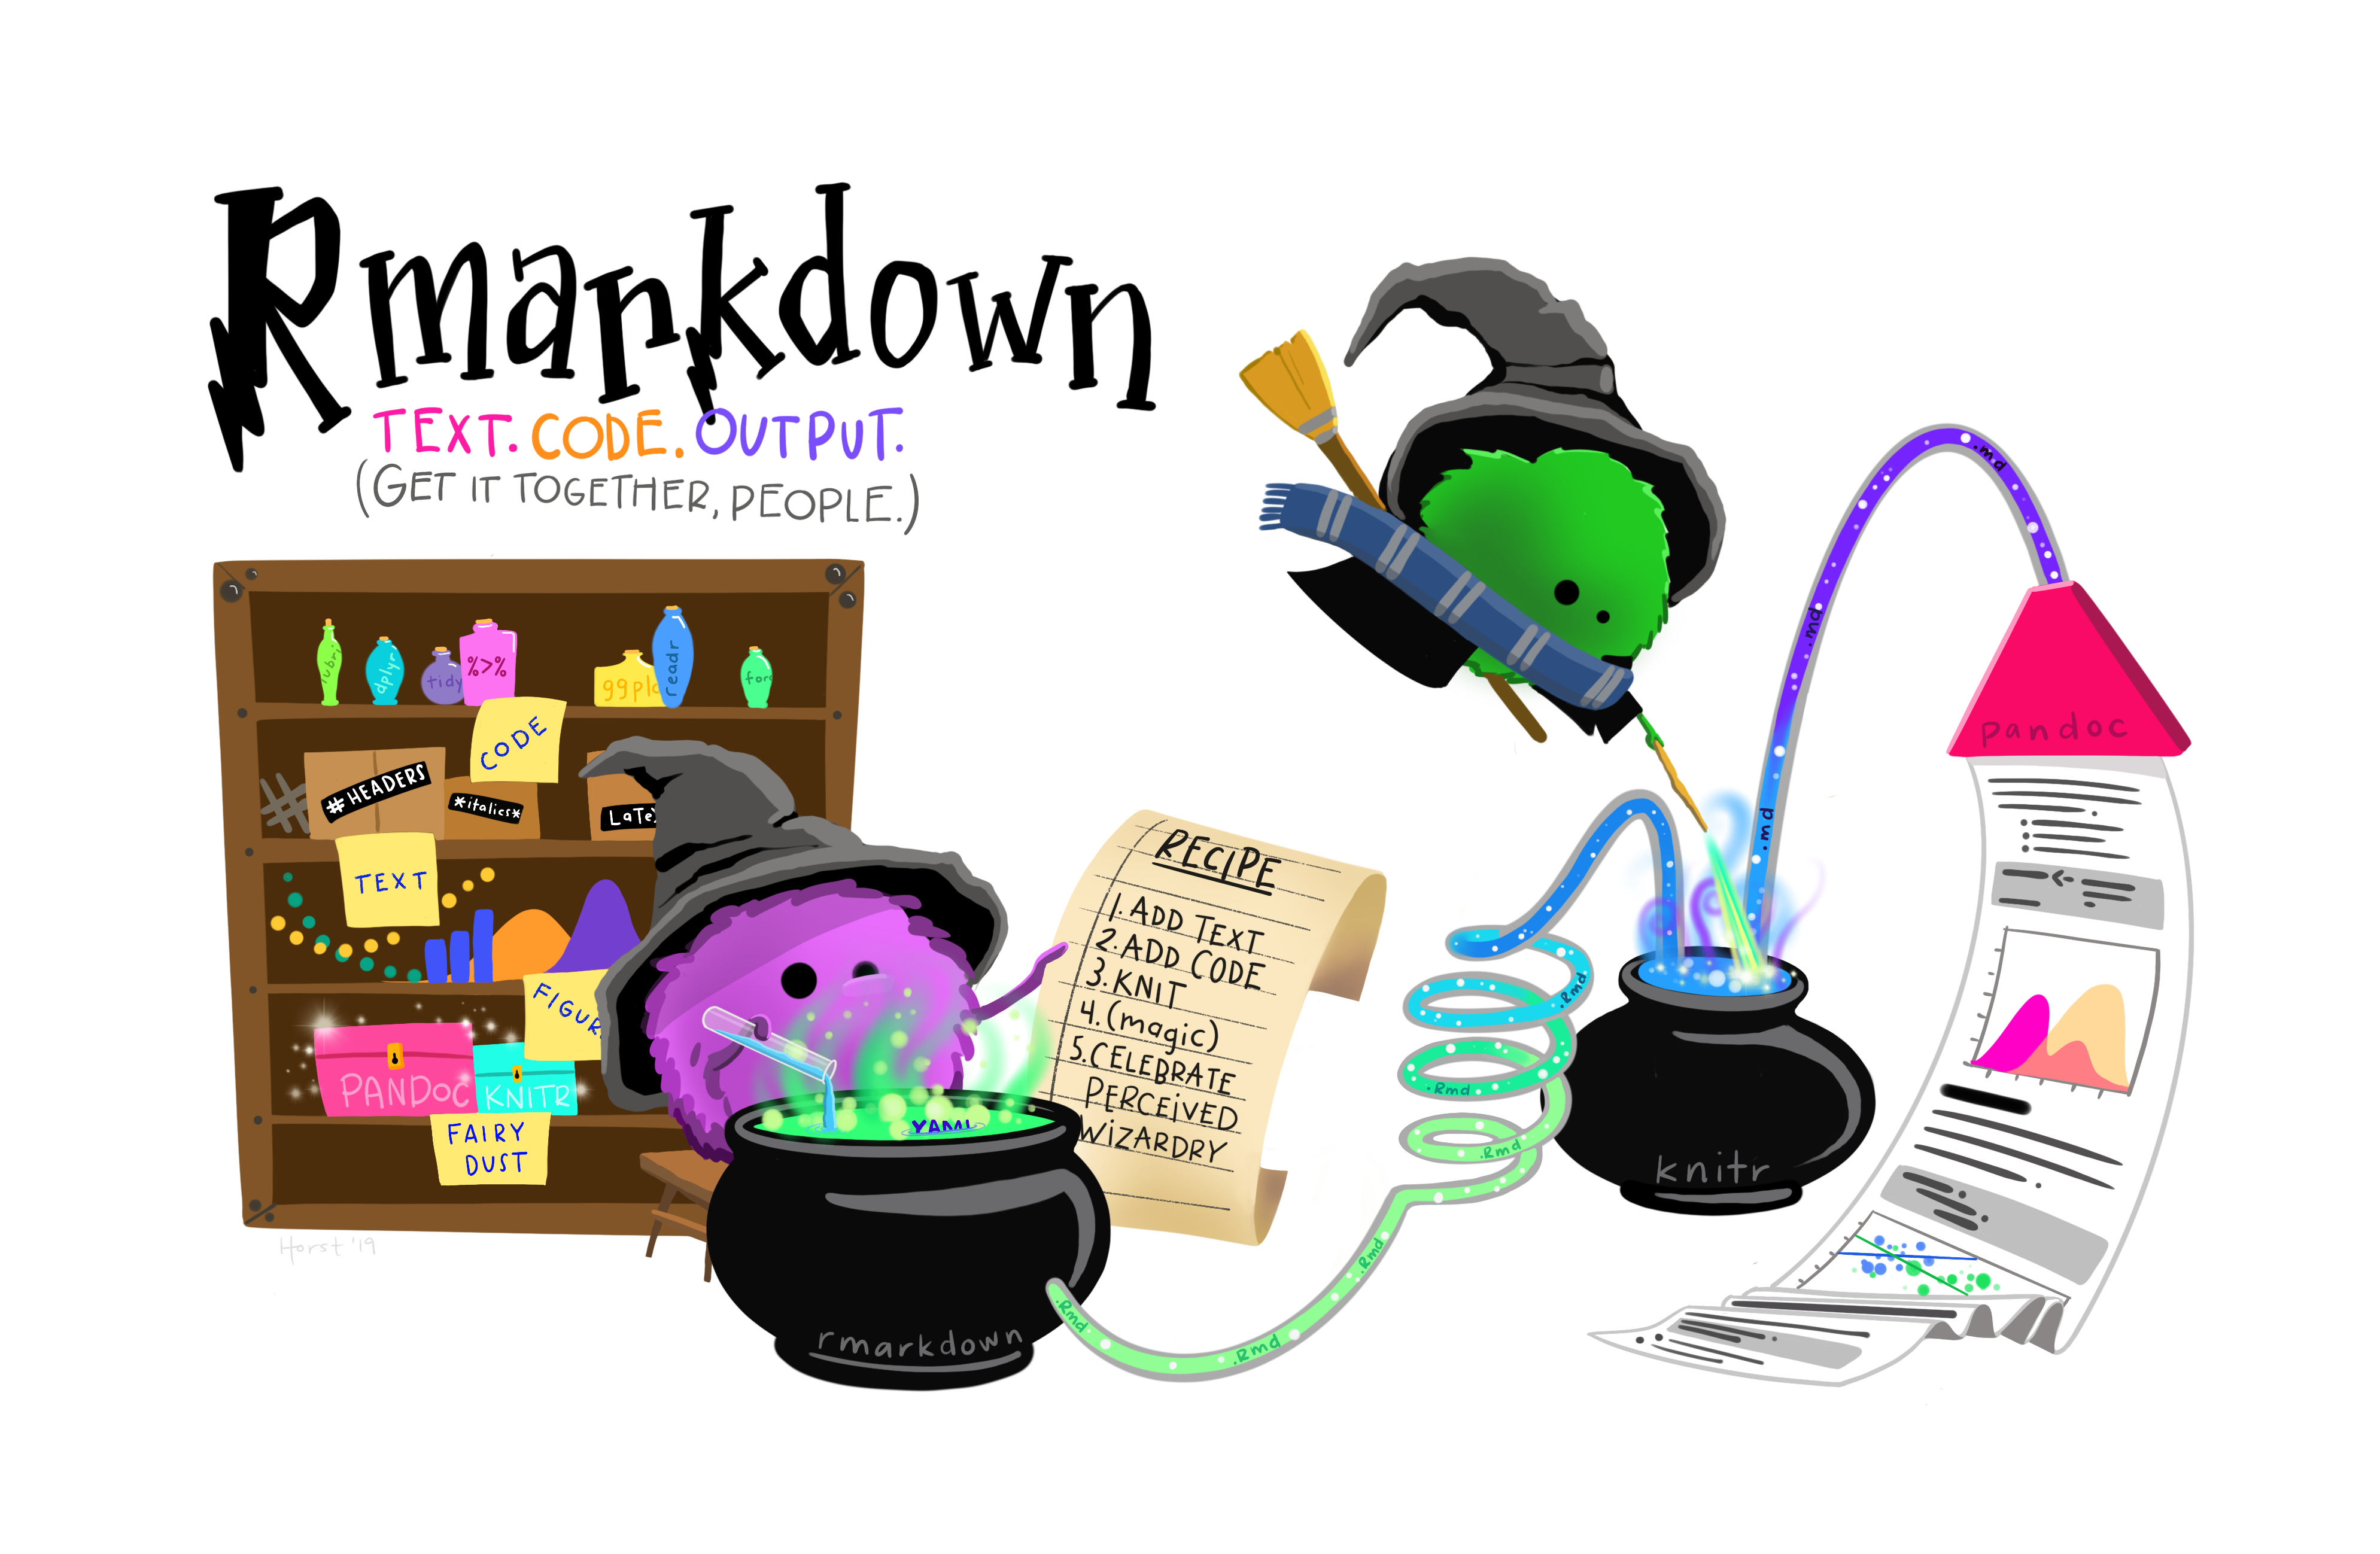
\includegraphics[width=55.24in]{img/rmarkdown_wizards} \caption{Artwork by allison horst}\label{fig:unnamed-chunk-39}
\end{figure}

\textbf{RMarkdown} is an authoring format that enables easy creation of dynamic documents, presentations, and reports from R. It combines markdown syntax with embedded R code chunks that are run so their output can be included in the final document.

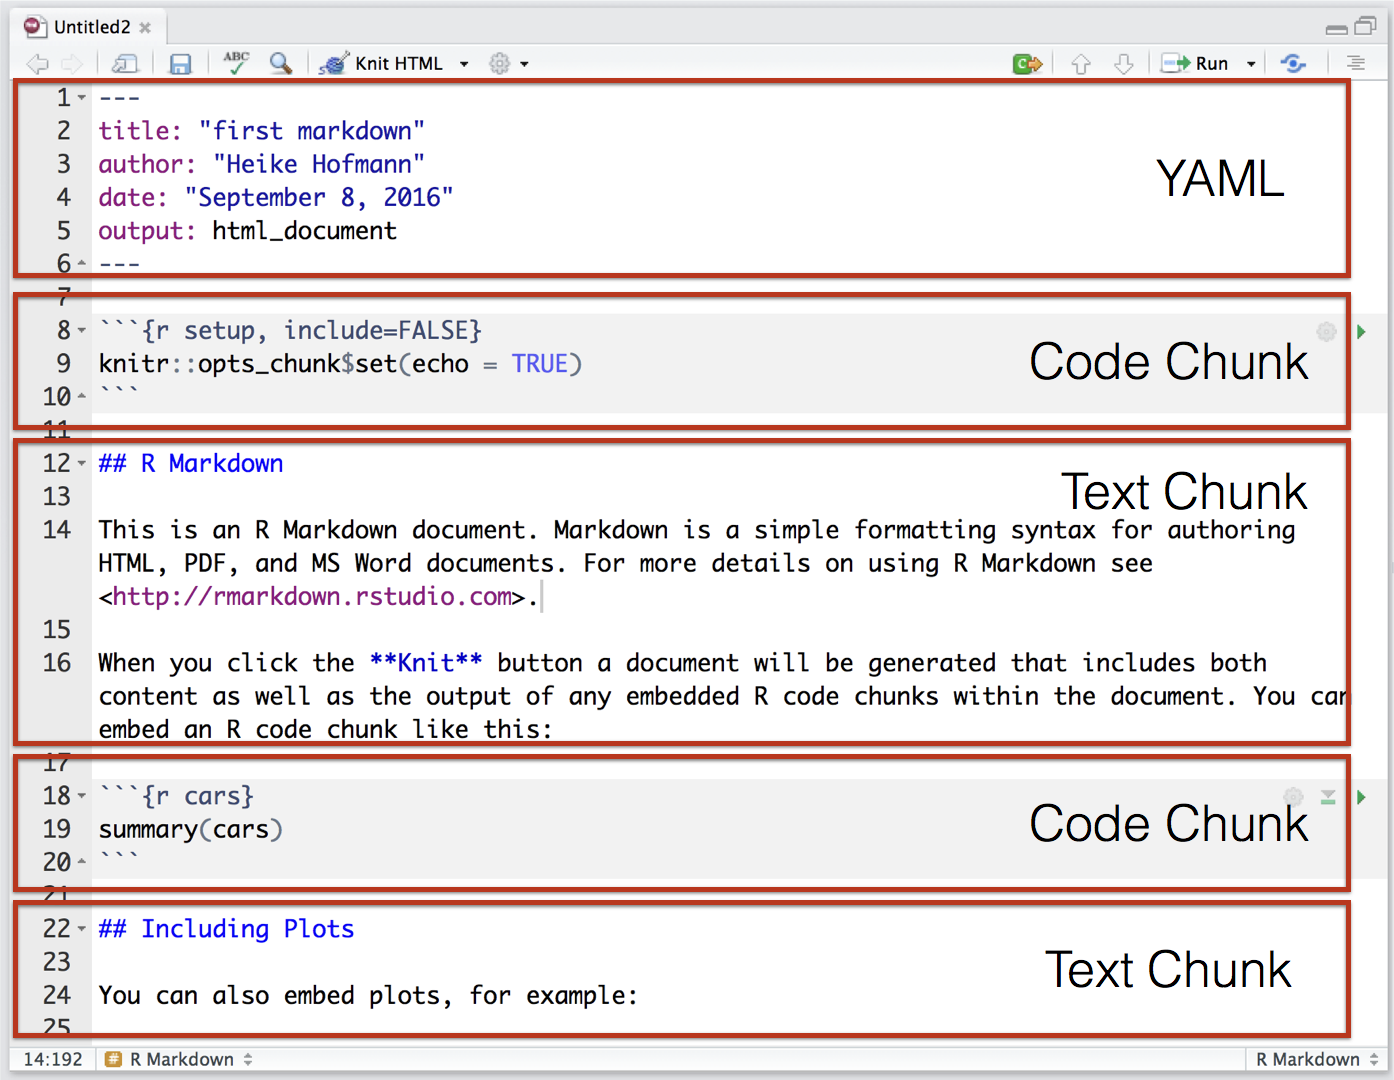
\includegraphics[width=19.36in]{img/rmarkdown}

Most importantly, RMarkdown creates fully reproducible reports since each time you knit the analysis is run from the beginning, encouraging transparency. Collaborators (including your future self) will thank you for integrating your analysis and report.

For a more in depth introduction, see \href{https://www.dataquest.io/blog/r-markdown-guide-cheatsheet/?utm_source=rbloggers\&utm_medium=referral\&utm_campaign=affiliate}{Getting Started with R Markdown --- Guide and Cheatsheet}, and to expand on your introduction, see \href{https://www.dataquest.io/blog/r-markdown-tips-tricks-and-shortcuts/?utm_source=rbloggers\&utm_medium=referral\&utm_campaign=affiliate}{R Markdown tips, tricks, and shortcuts}.

\hypertarget{exercise-create-your-first-rmarkdown.}{%
\subsubsection*{Exercise: Create your first Rmarkdown.}\label{exercise-create-your-first-rmarkdown.}}
\addcontentsline{toc}{subsubsection}{Exercise: Create your first Rmarkdown.}

\begin{enumerate}
\def\labelenumi{\arabic{enumi}.}
\tightlist
\item
  Open RStudio, create a new project.
\item
  Create a new RMarkdown file and knit it.
\item
  Make changes to the markdown formatting and knit again (use the \href{https://www.rstudio.com/resources/cheatsheets/}{RMarkdown cheat sheet})
\item
  If you feel adventurous, change some of the R code and knit again.
\end{enumerate}

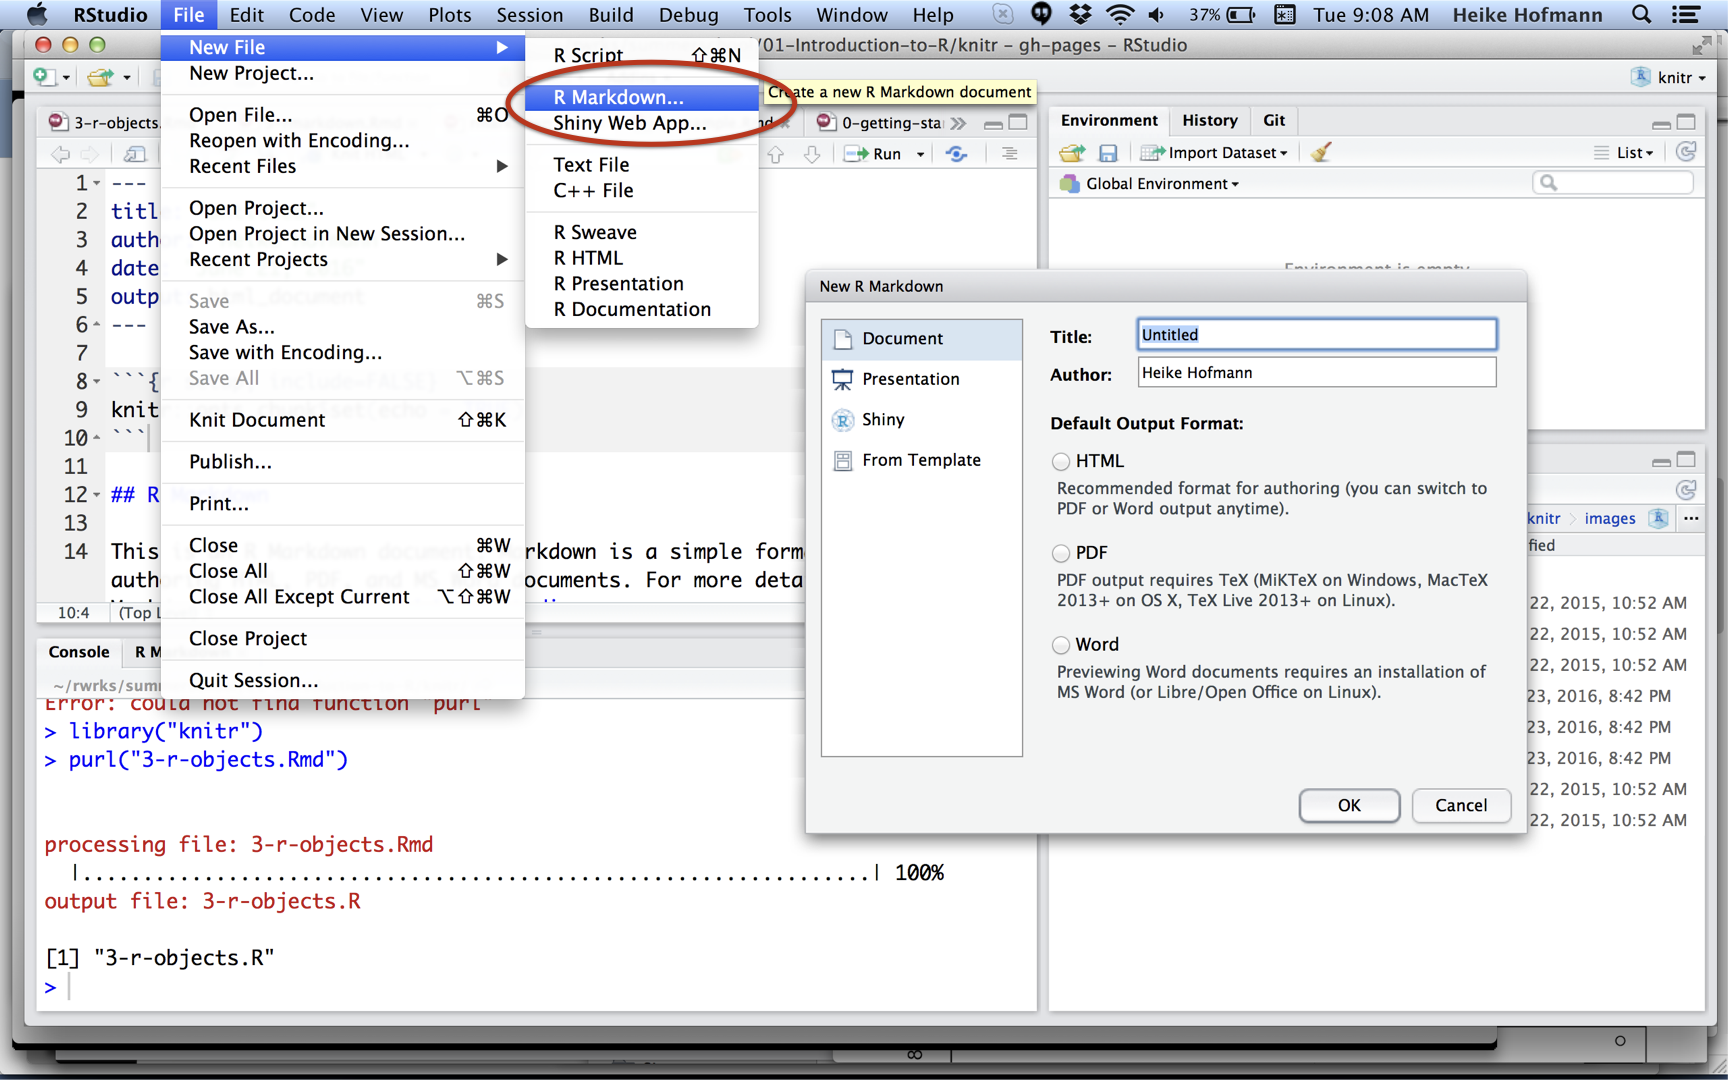
\includegraphics[width=24in]{img/hello-rmarkdown}

\hypertarget{graphics}{%
\chapter{Graphics}\label{graphics}}

\hypertarget{outline}{%
\section*{Outline}\label{outline}}
\addcontentsline{toc}{section}{Outline}

\hypertarget{introduction-to-ggplot2}{%
\paragraph*{1. Introduction to ggplot2}\label{introduction-to-ggplot2}}
\addcontentsline{toc}{paragraph}{1. Introduction to ggplot2}

\begin{itemize}
\tightlist
\item
  setup
\item
  why ggplot2
\item
  the evolution of a ggplot
\item
  create your first ggplot
\end{itemize}

\hypertarget{ggplot2-concepts}{%
\paragraph*{2. ggplot2 concepts}\label{ggplot2-concepts}}
\addcontentsline{toc}{paragraph}{2. ggplot2 concepts}

\begin{itemize}
\tightlist
\item
  the grammar of ggplot2
\item
  geometrical layers
\item
  statistical layers
\item
  facets
\item
  ggplots as objects
\end{itemize}

\hypertarget{advanced-customization}{%
\paragraph*{3. Advanced customization}\label{advanced-customization}}
\addcontentsline{toc}{paragraph}{3. Advanced customization}

\begin{itemize}
\tightlist
\item
  scales
\item
  coordinates
\item
  labels
\item
  annotations
\item
  themes
\item
  legends
\item
  fonts
\end{itemize}

\hypertarget{extensions}{%
\paragraph*{4. Extensions}\label{extensions}}
\addcontentsline{toc}{paragraph}{4. Extensions}

\begin{itemize}
\tightlist
\item
  patchwork
\item
  gganimate
\item
  ggplotly
\item
  ggiraph
\end{itemize}

\hypertarget{an-example}{%
\section{An example}\label{an-example}}

The data is a stratified sample of 70 students from a large section course. The strata were based on the college the students belonged to (AS = Arts \& Sciences, PM = Professional Management, MC = Mass Communications, and NU=Nursing) and their year in school (ranging from 1st to 3rd based on credit hours, and limited based on expectation of having at least 10 students from that college at that grade level). The response variables are their Hmwk = Homework Average and E1 to E3 = their grades on the first three exams.

\begin{Shaded}
\begin{Highlighting}[]
\FunctionTok{library}\NormalTok{(ggplot2)}
\NormalTok{url }\OtherTok{\textless{}{-}} \StringTok{"https://raw.githubusercontent.com/haleyjeppson/R4QM/main/data/CourseData.txt"}
\NormalTok{students }\OtherTok{\textless{}{-}}\NormalTok{ readr}\SpecialCharTok{::}\FunctionTok{read\_table}\NormalTok{(url)[, }\SpecialCharTok{{-}}\DecValTok{1}\NormalTok{]}
\NormalTok{students}
\end{Highlighting}
\end{Shaded}

\begin{verbatim}
## # A tibble: 70 x 6
##    College  Year  Hmwk    E1    E2    E3
##    <chr>   <dbl> <dbl> <dbl> <dbl> <dbl>
##  1 NU          1  83.8    79    89    59
##  2 NU          1  77.1    60    97    63
##  3 NU          1  94.5    83    88    69
##  4 NU          1  84.3    91    77    72
##  5 NU          1  73.4    68    79    76
##  6 NU          1  94.7    89    96    79
##  7 NU          1  77.7    76    43    84
##  8 NU          1  92.9    92    81    84
##  9 NU          1  95.9    84    85    84
## 10 NU          1  98.2    99    84    85
## # ... with 60 more rows
\end{verbatim}

\begin{Shaded}
\begin{Highlighting}[]
\FunctionTok{ggplot}\NormalTok{(students, }\FunctionTok{aes}\NormalTok{(College, E1)) }\SpecialCharTok{+}
  \FunctionTok{geom\_boxplot}\NormalTok{(}\FunctionTok{aes}\NormalTok{(}\AttributeTok{fill =} \FunctionTok{stage}\NormalTok{(College, }\AttributeTok{after\_scale =} \FunctionTok{alpha}\NormalTok{(fill, }\FloatTok{0.8}\NormalTok{))), }\AttributeTok{show.legend =} \ConstantTok{FALSE}\NormalTok{) }\SpecialCharTok{+}
  \FunctionTok{facet\_grid}\NormalTok{(}\SpecialCharTok{\textasciitilde{}}\NormalTok{Year, }\AttributeTok{scales =} \StringTok{"free"}\NormalTok{, }\AttributeTok{space =} \StringTok{"free\_x"}\NormalTok{, }\AttributeTok{labeller =} \FunctionTok{labeller}\NormalTok{(}\AttributeTok{Year =}\NormalTok{ label\_both)) }\SpecialCharTok{+}
  \FunctionTok{theme\_bw}\NormalTok{() }\SpecialCharTok{+}
  \FunctionTok{scale\_fill\_manual}\NormalTok{(}\AttributeTok{values =} \FunctionTok{c}\NormalTok{(}\StringTok{"\#69cadf"}\NormalTok{, }\StringTok{"\#f4602a"}\NormalTok{, }\StringTok{"\#fbb03b"}\NormalTok{, }\StringTok{"\#3273c2"}\NormalTok{))}
\end{Highlighting}
\end{Shaded}

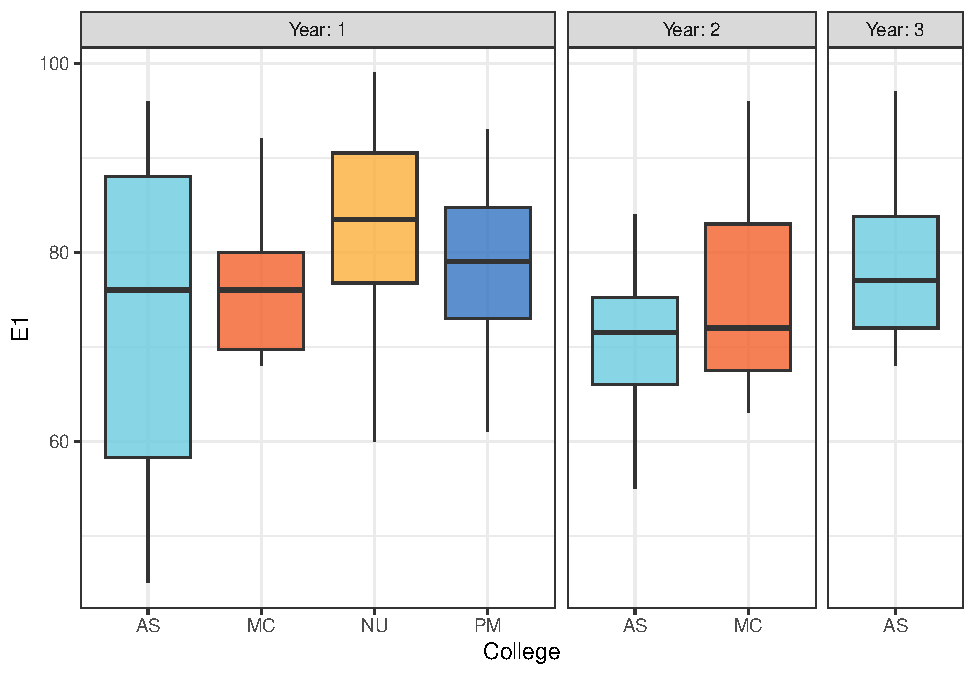
\includegraphics{_main_files/figure-latex/unnamed-chunk-44-1.pdf}

\hypertarget{transforming-data}{%
\chapter{Transforming Data}\label{transforming-data}}

\hypertarget{dplyr-basics}{%
\section*{\texorpdfstring{\texttt{\{dplyr\}} basics}{\{dplyr\} basics}}\label{dplyr-basics}}
\addcontentsline{toc}{section}{\texttt{\{dplyr\}} basics}

The book \href{https://r4ds.had.co.nz/}{R for Data Science} is a \emph{very} helpful reference guide. \href{https://r4ds.had.co.nz/transform.html}{Chapter 5} covers many of the topics covered in this section, and may be useful as a resource later or to dive deeper into a topic.

Topics:

\begin{itemize}
\tightlist
\item
  Filter rows

  \begin{itemize}
  \tightlist
  \item
    Comparisons
  \item
    Logical operators
  \item
    Missing values
  \end{itemize}
\item
  Arrange rows
\item
  Select columns
\item
  Add new variables
\item
  Grouped summaries

  \begin{itemize}
  \tightlist
  \item
    Combining multiple operations with the pipe
  \item
    Missing values
  \item
    Counts
  \item
    Useful summary functions
  \item
    Grouping by multiple variables
  \item
    Ungrouping
  \end{itemize}
\item
  Grouped mutates (and filters)
\item
  Extra: Working with factor variables
\end{itemize}

\hypertarget{an-example-1}{%
\section{An example}\label{an-example-1}}

The following example ties several of the above ideas together. Imagine that we have a set of grades from a course that we would like to convert to letter grades using a particular weighting and letter-grade cut-offs.

\begin{Shaded}
\begin{Highlighting}[]
\NormalTok{url }\OtherTok{\textless{}{-}} \StringTok{"https://raw.githubusercontent.com/haleyjeppson/R4QM/main/data/CourseData.txt"}
\NormalTok{students }\OtherTok{\textless{}{-}}\NormalTok{ readr}\SpecialCharTok{::}\FunctionTok{read\_table}\NormalTok{(url)[, }\SpecialCharTok{{-}}\DecValTok{1}\NormalTok{]}
\NormalTok{students}
\end{Highlighting}
\end{Shaded}

\begin{verbatim}
## # A tibble: 70 x 6
##    College  Year  Hmwk    E1    E2    E3
##    <chr>   <dbl> <dbl> <dbl> <dbl> <dbl>
##  1 NU          1  83.8    79    89    59
##  2 NU          1  77.1    60    97    63
##  3 NU          1  94.5    83    88    69
##  4 NU          1  84.3    91    77    72
##  5 NU          1  73.4    68    79    76
##  6 NU          1  94.7    89    96    79
##  7 NU          1  77.7    76    43    84
##  8 NU          1  92.9    92    81    84
##  9 NU          1  95.9    84    85    84
## 10 NU          1  98.2    99    84    85
## # ... with 60 more rows
\end{verbatim}

\begin{Shaded}
\begin{Highlighting}[]
\FunctionTok{head}\NormalTok{(students)}
\end{Highlighting}
\end{Shaded}

\begin{verbatim}
## # A tibble: 6 x 6
##   College  Year  Hmwk    E1    E2    E3
##   <chr>   <dbl> <dbl> <dbl> <dbl> <dbl>
## 1 NU          1  83.8    79    89    59
## 2 NU          1  77.1    60    97    63
## 3 NU          1  94.5    83    88    69
## 4 NU          1  84.3    91    77    72
## 5 NU          1  73.4    68    79    76
## 6 NU          1  94.7    89    96    79
\end{verbatim}

\begin{Shaded}
\begin{Highlighting}[]
\FunctionTok{tail}\NormalTok{(students)}
\end{Highlighting}
\end{Shaded}

\begin{verbatim}
## # A tibble: 6 x 6
##   College  Year  Hmwk    E1    E2    E3
##   <chr>   <dbl> <dbl> <dbl> <dbl> <dbl>
## 1 MC          2  83.2    69    77    93
## 2 MC          2  95.7    88    89    92
## 3 MC          2  79.3    80    61    97
## 4 MC          2  78.1    69    89    97
## 5 MC          2  99.1    84    89    96
## 6 MC          2  95.8    96   100   100
\end{verbatim}

In this particular case we want the weighting to be:

\begin{itemize}
\tightlist
\item
  20\% to Hmwk (col 3)
\item
  25\% to E1 (col 4)
\item
  25\% to E2 (col 5)
\item
  30\% to E3 (col 6)
\end{itemize}

But those weights could change later. A function can be written to take the data, and the weights and calculate the weighted average. We can then add that score to the students data frame, and add a final column with the actual letter grades on a 90-80-70-60 scale.

\begin{Shaded}
\begin{Highlighting}[]
\NormalTok{students }\OtherTok{\textless{}{-}}\NormalTok{ students }\SpecialCharTok{\%\textgreater{}\%} 
  \FunctionTok{mutate}\NormalTok{(}\AttributeTok{Final =}\NormalTok{ .}\DecValTok{2}\SpecialCharTok{*}\NormalTok{Hmwk }\SpecialCharTok{+}\NormalTok{ .}\DecValTok{25}\SpecialCharTok{*}\NormalTok{E1 }\SpecialCharTok{+}\NormalTok{ .}\DecValTok{25}\SpecialCharTok{*}\NormalTok{E2 }\SpecialCharTok{+}\NormalTok{ .}\DecValTok{3}\SpecialCharTok{*}\NormalTok{E3,}
         \AttributeTok{Grade =} \FunctionTok{case\_when}\NormalTok{(}
\NormalTok{           Final }\SpecialCharTok{\textless{}} \DecValTok{60} \SpecialCharTok{\textasciitilde{}} \StringTok{"F"}\NormalTok{,}
\NormalTok{           Final }\SpecialCharTok{\textless{}} \DecValTok{69} \SpecialCharTok{\textasciitilde{}} \StringTok{"D"}\NormalTok{,}
\NormalTok{           Final }\SpecialCharTok{\textless{}} \DecValTok{79} \SpecialCharTok{\textasciitilde{}} \StringTok{"C"}\NormalTok{,}
\NormalTok{           Final }\SpecialCharTok{\textless{}} \DecValTok{89} \SpecialCharTok{\textasciitilde{}} \StringTok{"B"}\NormalTok{,}
\NormalTok{           Final }\SpecialCharTok{\textgreater{}=} \DecValTok{90} \SpecialCharTok{\textasciitilde{}} \StringTok{"A"}\NormalTok{))}

\FunctionTok{head}\NormalTok{(students)}
\end{Highlighting}
\end{Shaded}

\begin{verbatim}
## # A tibble: 6 x 8
##   College  Year  Hmwk    E1    E2    E3 Final Grade
##   <chr>   <dbl> <dbl> <dbl> <dbl> <dbl> <dbl> <chr>
## 1 NU          1  83.8    79    89    59  76.5 C    
## 2 NU          1  77.1    60    97    63  73.6 C    
## 3 NU          1  94.5    83    88    69  82.4 B    
## 4 NU          1  84.3    91    77    72  80.5 B    
## 5 NU          1  73.4    68    79    76  74.2 C    
## 6 NU          1  94.7    89    96    79  88.9 B
\end{verbatim}

\hypertarget{reshaping-data}{%
\chapter{Reshaping Data}\label{reshaping-data}}

\hypertarget{tidyr-basics}{%
\section*{\texorpdfstring{\texttt{\{tidyr\}} basics}{\{tidyr\} basics}}\label{tidyr-basics}}
\addcontentsline{toc}{section}{\texttt{\{tidyr\}} basics}

The book \href{https://r4ds.had.co.nz/}{R for Data Science} is a \emph{very} helpful reference guide. \href{https://r4ds.had.co.nz/tidy-data.html}{Chapter 12} covers many of the topics covered in this section, and may be useful as a resource later or to dive deeper into a topic.

Topics:

\begin{itemize}
\tightlist
\item
  Tidy data
\item
  Pivoting

  \begin{itemize}
  \tightlist
  \item
    Longer
  \item
    Wider
  \end{itemize}
\item
  Separate \& unite
\end{itemize}

\hypertarget{an-example-2}{%
\section{An example}\label{an-example-2}}

For this example we begin with a subset of the 2009 \href{https://nces.ed.gov/surveys/pisa/}{Program for International Student Assessment (PISA)} data.

\begin{Shaded}
\begin{Highlighting}[]
\DocumentationTok{\#\# load data}
\NormalTok{url }\OtherTok{\textless{}{-}} \StringTok{"https://raw.githubusercontent.com/haleyjeppson/R4QM/main/data/pisas09\_subset.csv"}
\NormalTok{pisas }\OtherTok{\textless{}{-}}\NormalTok{ readr}\SpecialCharTok{::}\FunctionTok{read\_csv}\NormalTok{(url)}
\NormalTok{pisas}
\end{Highlighting}
\end{Shaded}

\begin{verbatim}
## # A tibble: 475,460 x 5
##    country sex     math  read weight
##    <chr>   <chr>  <dbl> <dbl>  <dbl>
##  1 Albania Male    333.  279.   5.40
##  2 Albania Male    344.  327.   5.40
##  3 Albania Male    456.  423.   5.40
##  4 Albania Female  394.  420.   5.70
##  5 Albania Female  277.  375.   5.70
##  6 Albania Male    514.  544.   5.40
##  7 Albania Female  425.  477.   5.70
##  8 Albania Female  322.  339.   5.70
##  9 Albania Male    332.  319.   5.40
## 10 Albania Male    387.  430.   5.40
## # ... with 475,450 more rows
\end{verbatim}

\hypertarget{pivot-to-long-form}{%
\subsubsection*{Pivot to long form}\label{pivot-to-long-form}}
\addcontentsline{toc}{subsubsection}{Pivot to long form}

Say we want to compare math and reading scores across a subset of countries. To do so, we will need to reshape our data into long form:

\begin{Shaded}
\begin{Highlighting}[]
\DocumentationTok{\#\# in long form}
\NormalTok{pisas\_long }\OtherTok{\textless{}{-}}\NormalTok{ pisas }\SpecialCharTok{\%\textgreater{}\%} 
  \FunctionTok{select}\NormalTok{(}\SpecialCharTok{{-}}\NormalTok{sex) }\SpecialCharTok{\%\textgreater{}\%} 
  \FunctionTok{pivot\_longer}\NormalTok{(}\AttributeTok{cols =}\NormalTok{ math}\SpecialCharTok{:}\NormalTok{read, }\AttributeTok{names\_to =} \StringTok{"item"}\NormalTok{, }\AttributeTok{values\_to =} \StringTok{"score"}\NormalTok{)}
\NormalTok{pisas\_long}
\end{Highlighting}
\end{Shaded}

\begin{verbatim}
## # A tibble: 950,920 x 4
##    country weight item  score
##    <chr>    <dbl> <chr> <dbl>
##  1 Albania   5.40 math   333.
##  2 Albania   5.40 read   279.
##  3 Albania   5.40 math   344.
##  4 Albania   5.40 read   327.
##  5 Albania   5.40 math   456.
##  6 Albania   5.40 read   423.
##  7 Albania   5.70 math   394.
##  8 Albania   5.70 read   420.
##  9 Albania   5.70 math   277.
## 10 Albania   5.70 read   375.
## # ... with 950,910 more rows
\end{verbatim}

\begin{Shaded}
\begin{Highlighting}[]
\NormalTok{pisas\_long }\SpecialCharTok{\%\textgreater{}\%} 
  \FunctionTok{filter}\NormalTok{(country }\SpecialCharTok{\%in\%} \FunctionTok{c}\NormalTok{(}\StringTok{"Finland"}\NormalTok{, }\StringTok{"United States"}\NormalTok{)) }\SpecialCharTok{\%\textgreater{}\%}
  \FunctionTok{ggplot}\NormalTok{(}\FunctionTok{aes}\NormalTok{(}\AttributeTok{x =}\NormalTok{ score, }\AttributeTok{weight =}\NormalTok{ weight, }\AttributeTok{fill =}\NormalTok{ country)) }\SpecialCharTok{+}
  \FunctionTok{geom\_density}\NormalTok{(}\AttributeTok{alpha =} \FloatTok{0.6}\NormalTok{) }\SpecialCharTok{+}
  \FunctionTok{facet\_wrap}\NormalTok{(}\SpecialCharTok{\textasciitilde{}}\NormalTok{item) }\SpecialCharTok{+}
  \FunctionTok{theme\_bw}\NormalTok{() }\SpecialCharTok{+}
  \FunctionTok{scale\_fill\_manual}\NormalTok{(}\AttributeTok{values =} \FunctionTok{c}\NormalTok{(}\StringTok{"\#69cadf"}\NormalTok{, }\StringTok{"\#f4602a"}\NormalTok{, }\StringTok{"\#fbb03b"}\NormalTok{, }\StringTok{"\#3273c2"}\NormalTok{)[}\FunctionTok{c}\NormalTok{(}\DecValTok{3}\NormalTok{,}\DecValTok{1}\NormalTok{)]) }\SpecialCharTok{+}
  \FunctionTok{labs}\NormalTok{(}\AttributeTok{title =} \StringTok{"Distribution of PISA 2009 Scores"}\NormalTok{, }\AttributeTok{x =} \ConstantTok{NULL}\NormalTok{, }\AttributeTok{y =} \ConstantTok{NULL}\NormalTok{)}
\end{Highlighting}
\end{Shaded}

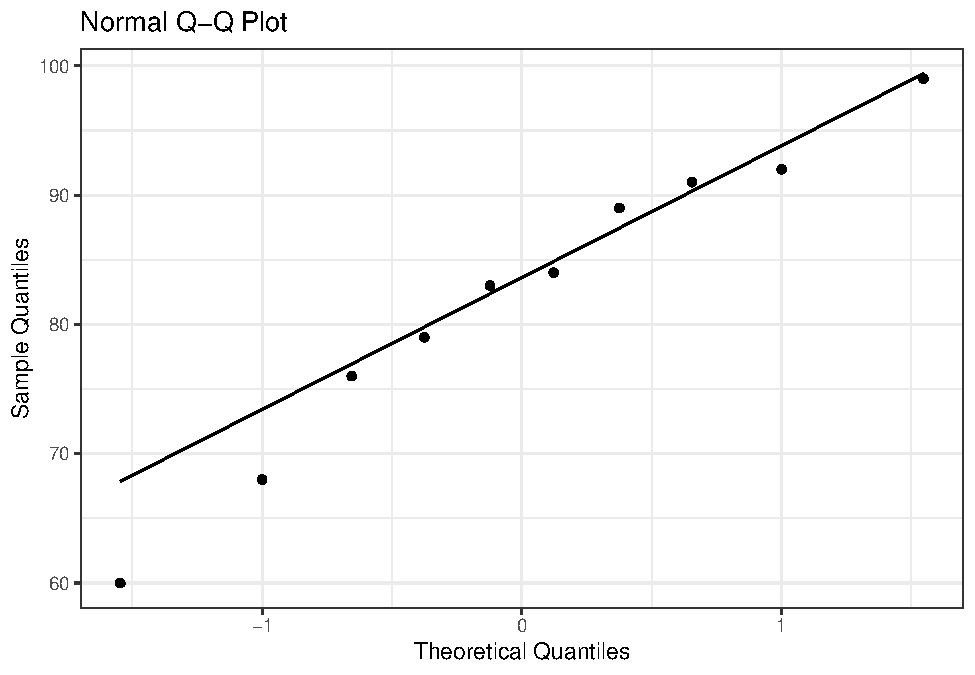
\includegraphics{_main_files/figure-latex/unnamed-chunk-49-1.pdf}

\hypertarget{pivot-to-wide-form}{%
\subsubsection*{Pivot to wide form}\label{pivot-to-wide-form}}
\addcontentsline{toc}{subsubsection}{Pivot to wide form}

Say we want to plot male math scores against female math scores. To do so, we will need to summarize our data and then reshape our data into a wider format:

\begin{Shaded}
\begin{Highlighting}[]
\DocumentationTok{\#\# in wide form}
\NormalTok{pisas\_wide }\OtherTok{\textless{}{-}}\NormalTok{ pisas }\SpecialCharTok{\%\textgreater{}\%} 
  \FunctionTok{select}\NormalTok{(}\SpecialCharTok{{-}}\NormalTok{read) }\SpecialCharTok{\%\textgreater{}\%} 
  \FunctionTok{group\_by}\NormalTok{(country, sex) }\SpecialCharTok{\%\textgreater{}\%} 
  \FunctionTok{summarise}\NormalTok{(}\AttributeTok{math =} \FunctionTok{weighted.mean}\NormalTok{(math, weight, }\AttributeTok{na.rm =} \ConstantTok{TRUE}\NormalTok{)) }\SpecialCharTok{\%\textgreater{}\%} 
  \FunctionTok{pivot\_wider}\NormalTok{(}\AttributeTok{names\_from =}\NormalTok{ sex, }\AttributeTok{values\_from =}\NormalTok{ math) }
  
\NormalTok{pisas\_wide}
\end{Highlighting}
\end{Shaded}

\begin{verbatim}
## # A tibble: 65 x 4
## # Groups:   country [65]
##    country    Female  Male  `NA`
##    <chr>       <dbl> <dbl> <dbl>
##  1 Albania      382.  372.    NA
##  2 Argentina    383.  393.    NA
##  3 Australia    510.  519.    NA
##  4 Austria      486.  505.    NA
##  5 Azerbaijan   426.  436.    NA
##  6 Belgium      505.  526.    NA
##  7 Brazil       378.  395.    NA
##  8 Bulgaria     431.  425.    NA
##  9 Canada       520.  532.    NA
## 10 Chile        410.  431.    NA
## # ... with 55 more rows
\end{verbatim}

\begin{Shaded}
\begin{Highlighting}[]
\FunctionTok{ggplot}\NormalTok{(pisas\_wide, }\FunctionTok{aes}\NormalTok{(}\AttributeTok{x =}\NormalTok{ Female, }\AttributeTok{y =}\NormalTok{ Male)) }\SpecialCharTok{+}
  \FunctionTok{geom\_abline}\NormalTok{(}\AttributeTok{alpha =} \FloatTok{0.2}\NormalTok{) }\SpecialCharTok{+}
  \FunctionTok{geom\_point}\NormalTok{() }\SpecialCharTok{+}
  \FunctionTok{labs}\NormalTok{(}\AttributeTok{title =} \StringTok{"PISA 2009 in Math {-} Gender Gap"}\NormalTok{,}
       \AttributeTok{x =} \StringTok{"PISA 2009 Math score for girls"}\NormalTok{,}
       \AttributeTok{y =} \StringTok{"PISA 2015 Math score for boys"}\NormalTok{) }\SpecialCharTok{+}
  \FunctionTok{theme\_light}\NormalTok{()}
\end{Highlighting}
\end{Shaded}

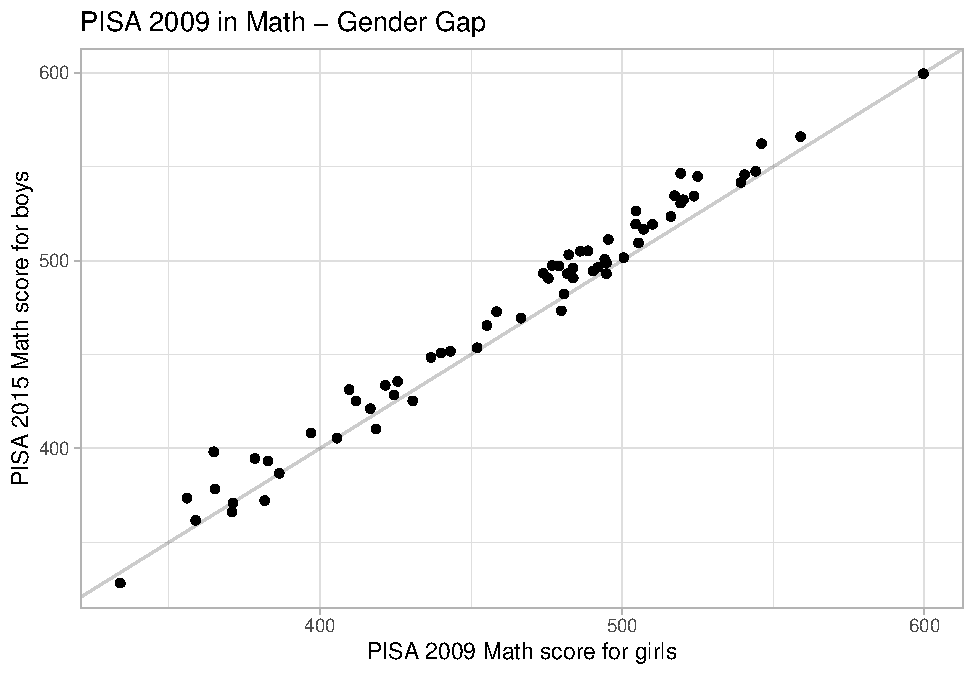
\includegraphics{_main_files/figure-latex/unnamed-chunk-50-1.pdf}

This book pulls from many sources, including:

\begin{itemize}
\item
  \href{https://r4ds.had.co.nz/}{R for Data Science}
\item
  \href{https://bookdown.org/yihui/rmarkdown-cookbook/}{R Markdown Cookbook}
\item
  \href{https://bookdown.org/yihui/bookdown/}{bookdown: Authoring Books and Technical Documents with R Markdown}
\item
  \href{https://stat480-at-isu.github.io/schedule.html}{Applied Statistical Computing}.
\item
  \href{https://people.stat.sc.edu/habing/RforQM/RforQM.htm}{An Introduction to R for Quantitative Methods}
\item
  \href{https://socviz.co/}{Data Visualization: A Practical Introduction}
\item
  \href{https://clauswilke.com/dataviz/index.html}{Fundamentals of Data Visualization}
\item
  \href{https://rstats.wtf/}{What They Forgot to Teach You About R}
\item
  \href{https://www.tmwr.org/}{Tidy Modeling with R}
\end{itemize}

\hypertarget{packages-1}{%
\section*{Packages}\label{packages-1}}
\addcontentsline{toc}{section}{Packages}

\begin{Shaded}
\begin{Highlighting}[]
\FunctionTok{subset}\NormalTok{(}\FunctionTok{data.frame}\NormalTok{(sessioninfo}\SpecialCharTok{::}\FunctionTok{package\_info}\NormalTok{()), attached}\SpecialCharTok{==}\ConstantTok{TRUE}\NormalTok{, }\FunctionTok{c}\NormalTok{(package, loadedversion))}
\end{Highlighting}
\end{Shaded}

\begin{verbatim}
##             package loadedversion
## dplyr         dplyr        1.0.10
## forcats     forcats         0.5.1
## ggplot2     ggplot2         3.4.0
## purrr         purrr         1.0.1
## readr         readr         2.1.2
## stringr     stringr         1.4.1
## tibble       tibble         3.1.8
## tidyr         tidyr         1.2.1
## tidyverse tidyverse         1.3.1
\end{verbatim}

  \bibliography{book.bib,packages.bib}

\end{document}
